\section{Controles} % 5.3 Controls

\change[inline]{Map out the game procedures and controls. Use visualizations
like control tables and flowcharts, along with descriptions.}

\subsection{Acciones}

\change[inline]{Las acciones son aquellas cosas que puede hacer el jugador
dentro del juego. Se agruparán según a qué modo pertenecen.}

La acción que podrá realizar el jugador en la mayoría de modos es:
\begin{itemize}
    \item Acceder a la configuración general
\end{itemize}
El único modo en el que no puede realizar esta acción es el modo partida.

\subsubsection{Modo menú principal}
\begin{itemize}
    \item Acceder al menú de selección de perfiles
    \item Salir del juego
\end{itemize}

\subsubsection{Modo selección de perfil}
\begin{itemize}
    \item Borrar perfil
    \item Crear perfil
    \item Entrar al perfil
    \item Volver al menú principal
\end{itemize}

\subsubsection{Modo perfil}
\begin{itemize}
    \item Crear nueva partida
    \item Cambiar configuracion de perfil
    \item Volver al menú de selección de perfil
\end{itemize}

\subsubsection{Modo configuración de partida}
\begin{itemize}
    \item Configurar datos de la partida
    \item Entrar al menú de selección de personaje
    \item Volver al perfil
\end{itemize}

\subsubsection{Modo selección de personaje}
\begin{itemize}
    \item Cambiar de personaje
    \item Seleccionar personaje
    \item Volver al menú de configuración de partida
\end{itemize}

\subsubsection{Modo partida}
\change[inline]{No se puede acceder al menú de configuración general desde aquí directamente}

\begin{itemize}
    \item Moverse
    \item Atacar
    \item Usar habilidad
    \item Usar objeto
    \item Recolectar objeto
    \item Descartar objeto
    \item Interactuar con NPC
    \item Comprar objeto
    \item Recolectar monedas
    \item Pausar
    \item Avanzar de nivel
\end{itemize}

\subsubsection{Modo pausa}
\begin{itemize}
    \item Abandonar partida
    \item Volver a la partida
\end{itemize}

\subsubsection{Modo victoria}
\begin{itemize}
    \item Salir de la partida
\end{itemize}

\subsubsection{Modo derrota}
\begin{itemize}
    \item Salir de la partida
\end{itemize}

\subsubsection{Modo configuración}
\begin{itemize}
    \item Cambiar el volumen de sonido
\end{itemize}

\subsection{Interacciones}
% Lo que hacen los NPCs y monstruos


\subsection{Condiciones de victoria/puntuación} % 5.3.3 Scoring/winning conditions

\change[inline]{Describe the scoring system and win conditions. These might be
different for single player versus multiplayer or if you have several modes of
competition.}

\subsection{Reglas} %     5.3.2 Rules

\change[inline]{If you have created a prototype, describing the rules of your
game will be much easier. You will need to define all the game objects,
concepts, their behaviors, and how they relate to one another in this section}

\subsection{Interfaces} %     5.3.1 Interfaces

\change[inline]{Create wireframes, as described on page 439, for every interface
the artists will need to create. Each wireframe should include a description of
how each interface feature functions. Make sure you detail out the various
states for each interface.}

\subsubsection{Modo menú principal}
\begin{figure}[H]
    \centering
    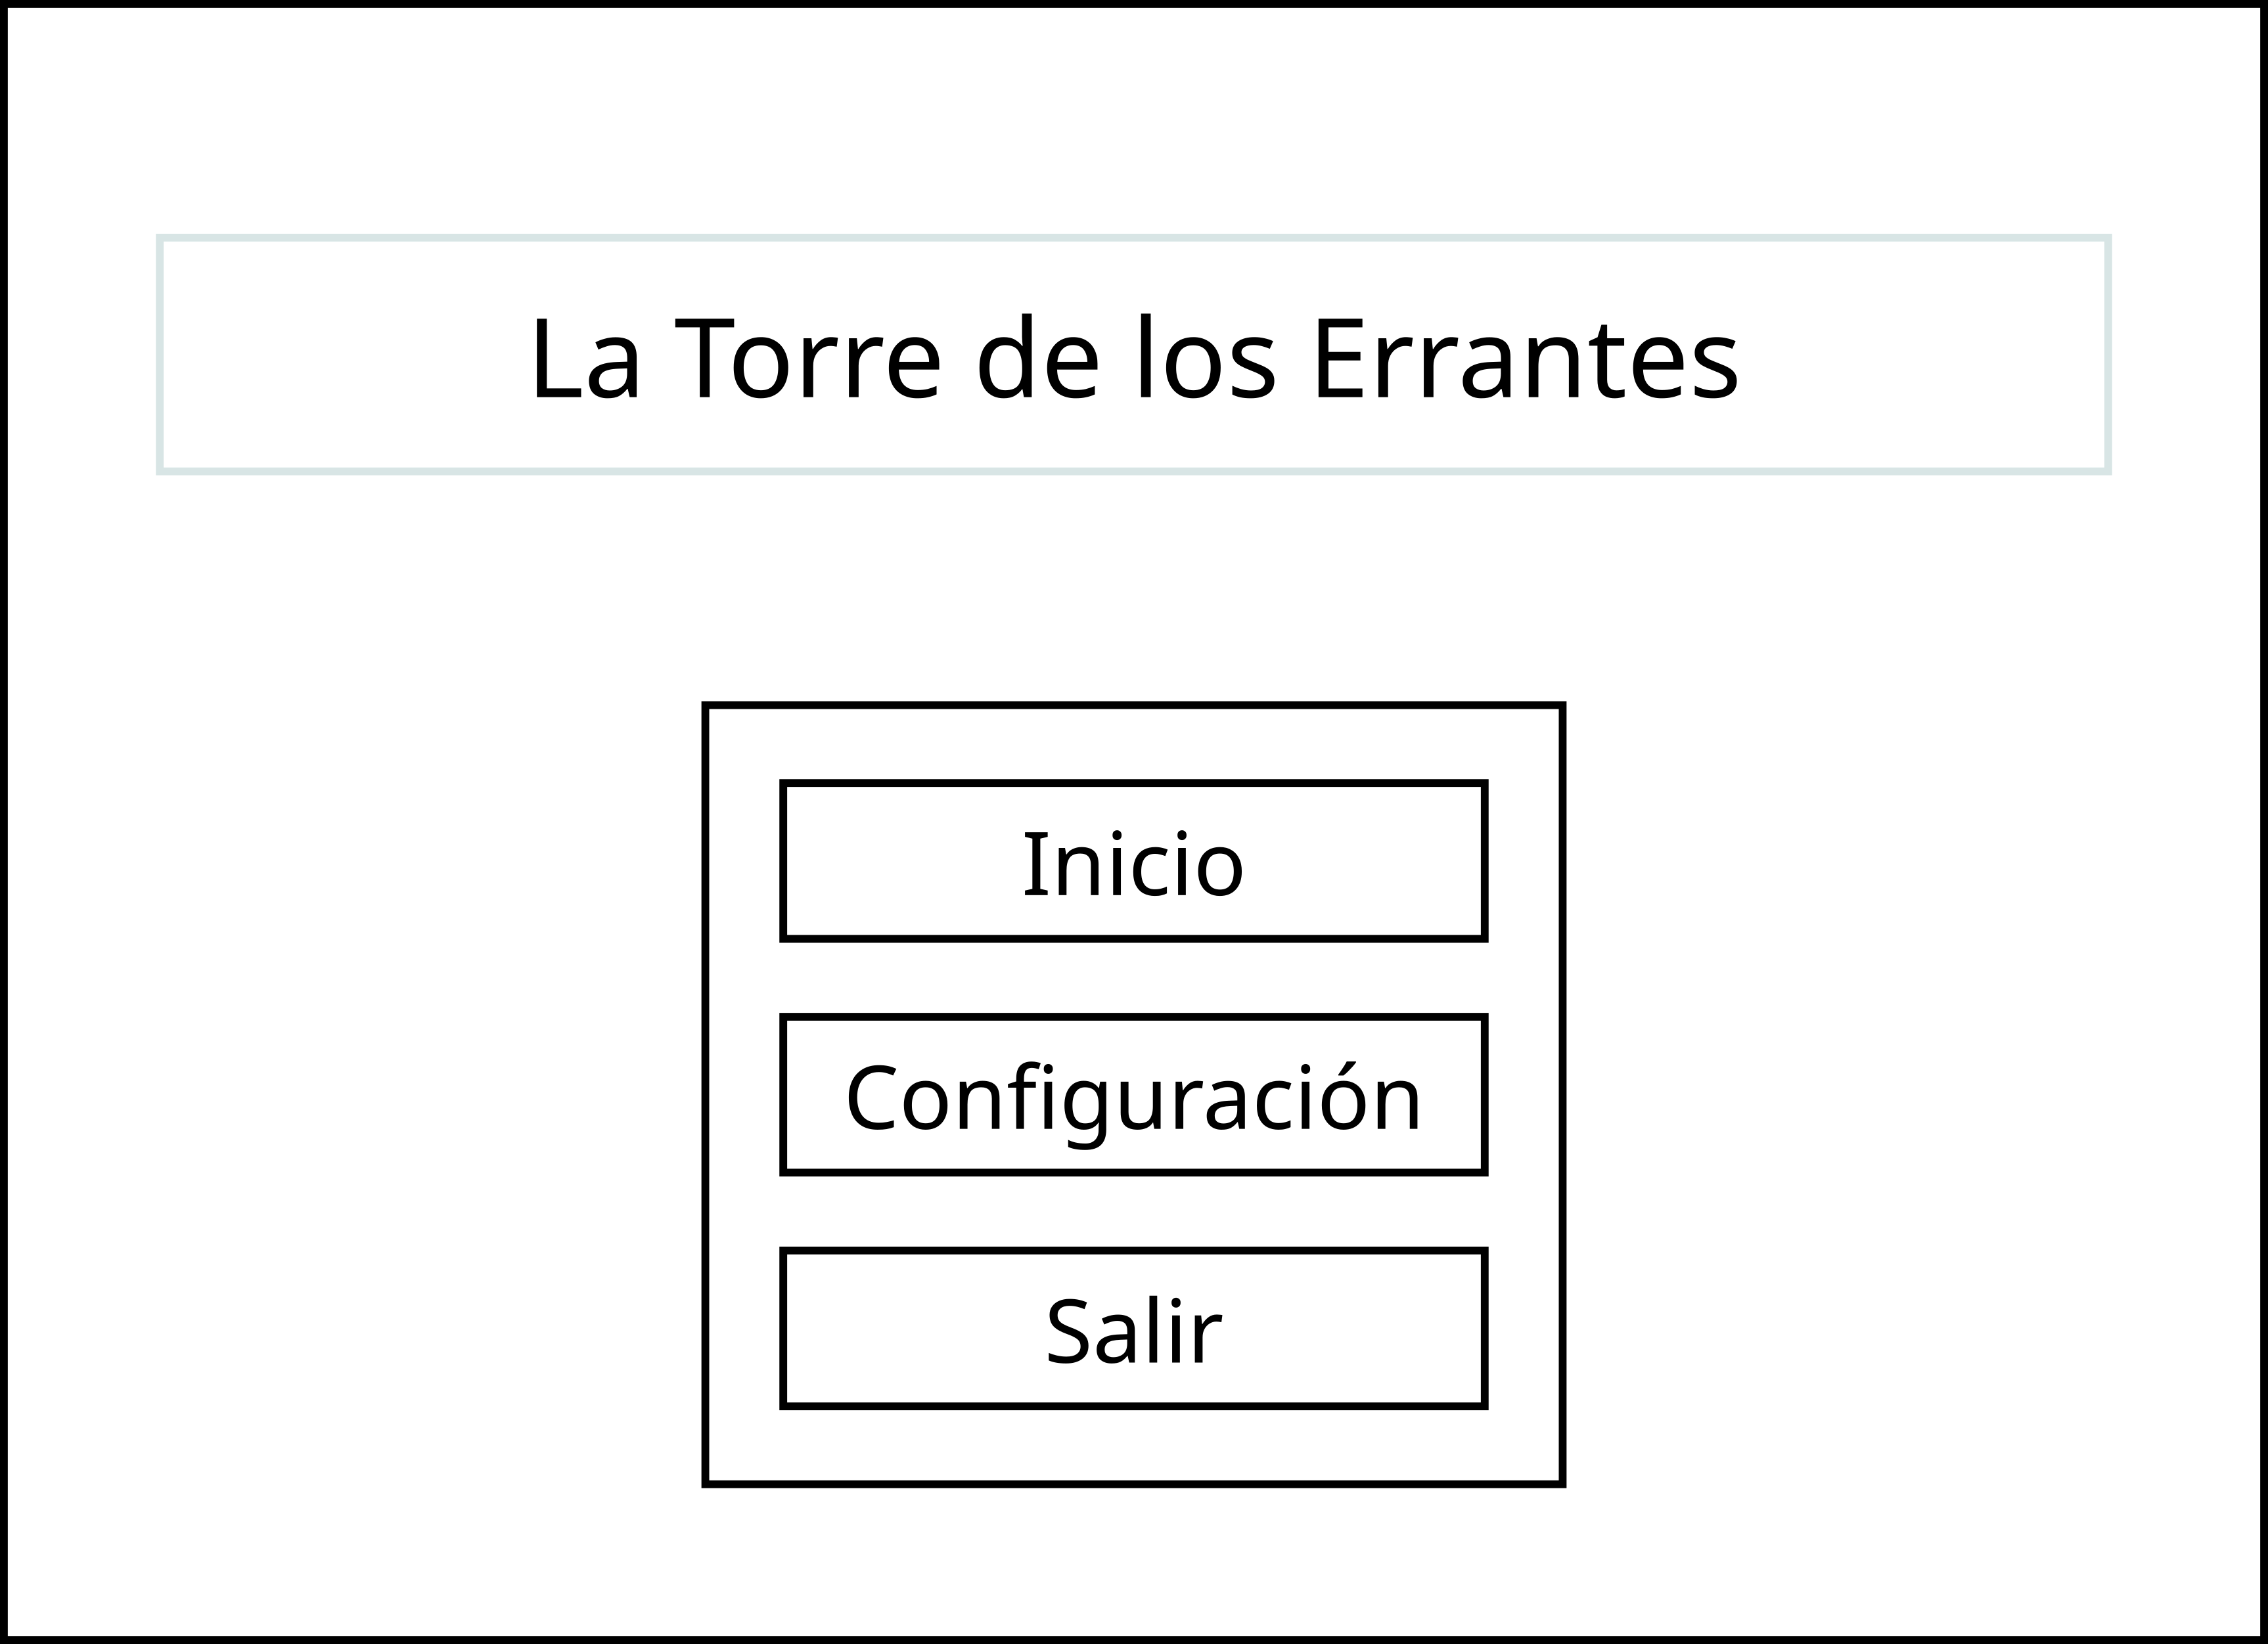
\includegraphics[width=0.5\textwidth]{5-Cuerpo/Chapter5/I1.png} %
    \caption{}
    \label{fig:I1}
\end{figure}

\subsubsection{Modo selección de perfil}
\begin{figure}[H]
    \centering
    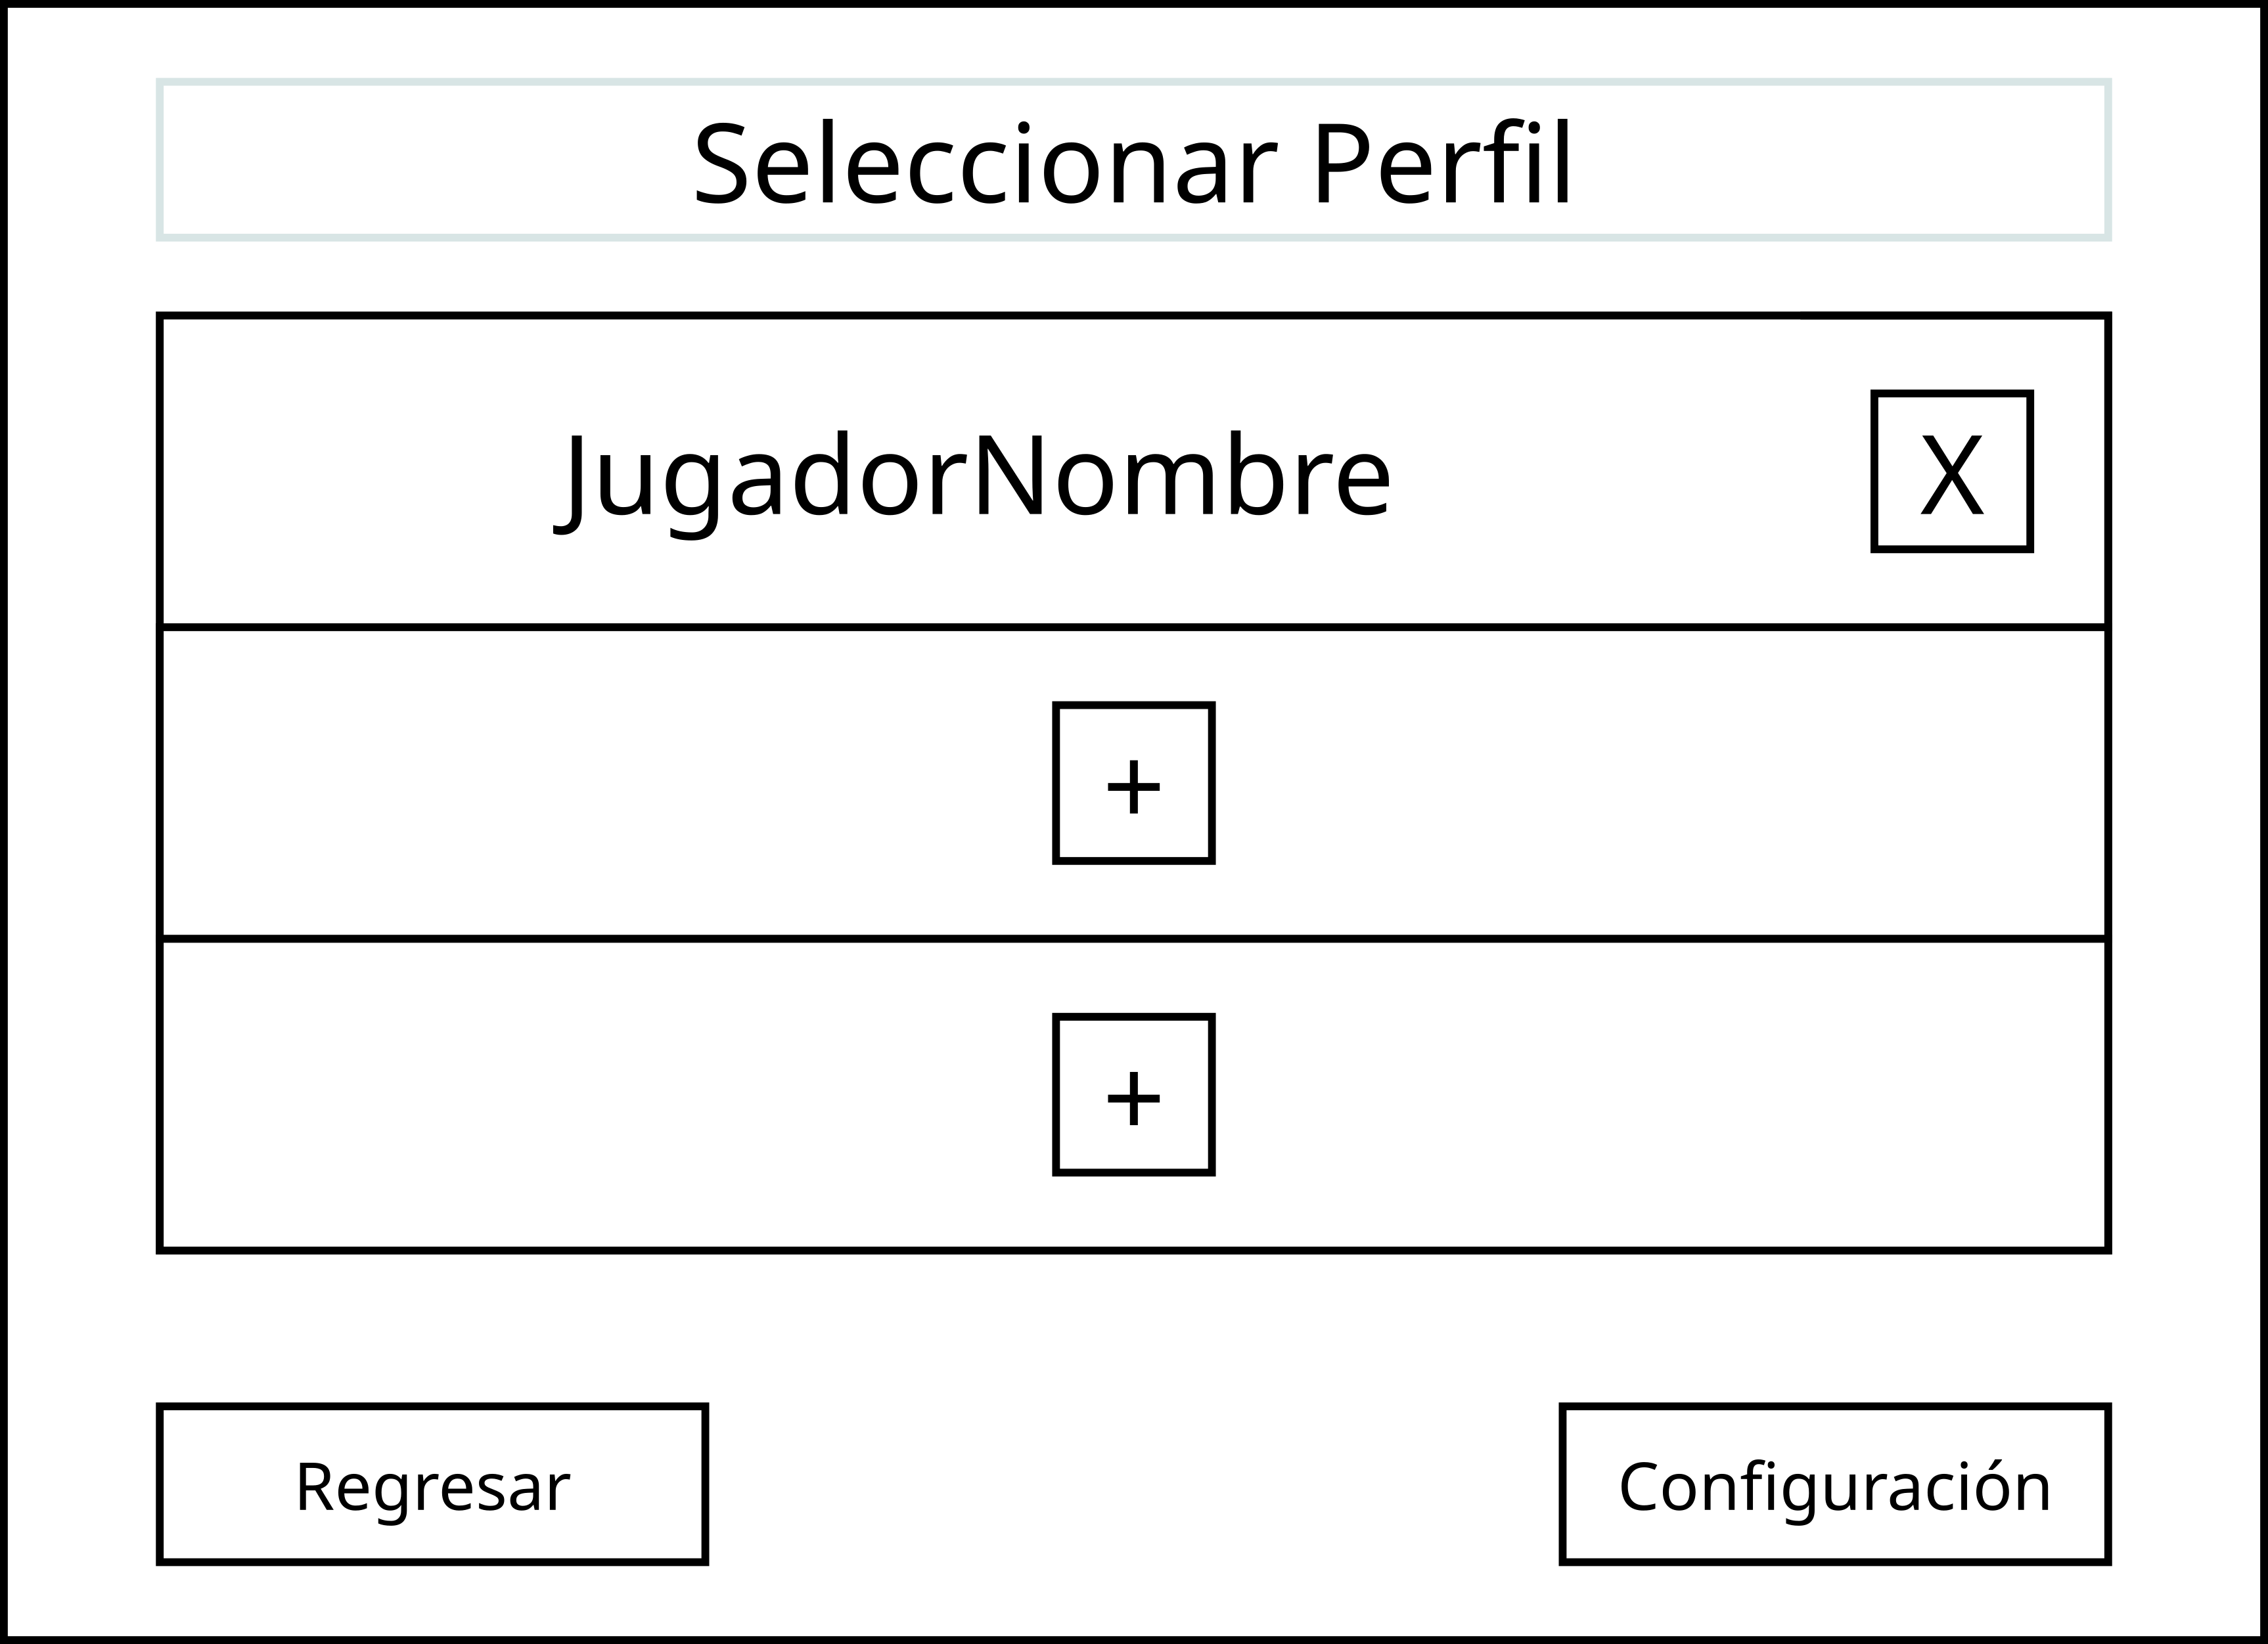
\includegraphics[width=0.5\textwidth]{5-Cuerpo/Chapter5/I3.png} %
    \caption{}
    \label{fig:I3}
\end{figure}

\subsubsection{Modo perfil}
\begin{figure}[H]
    \centering
    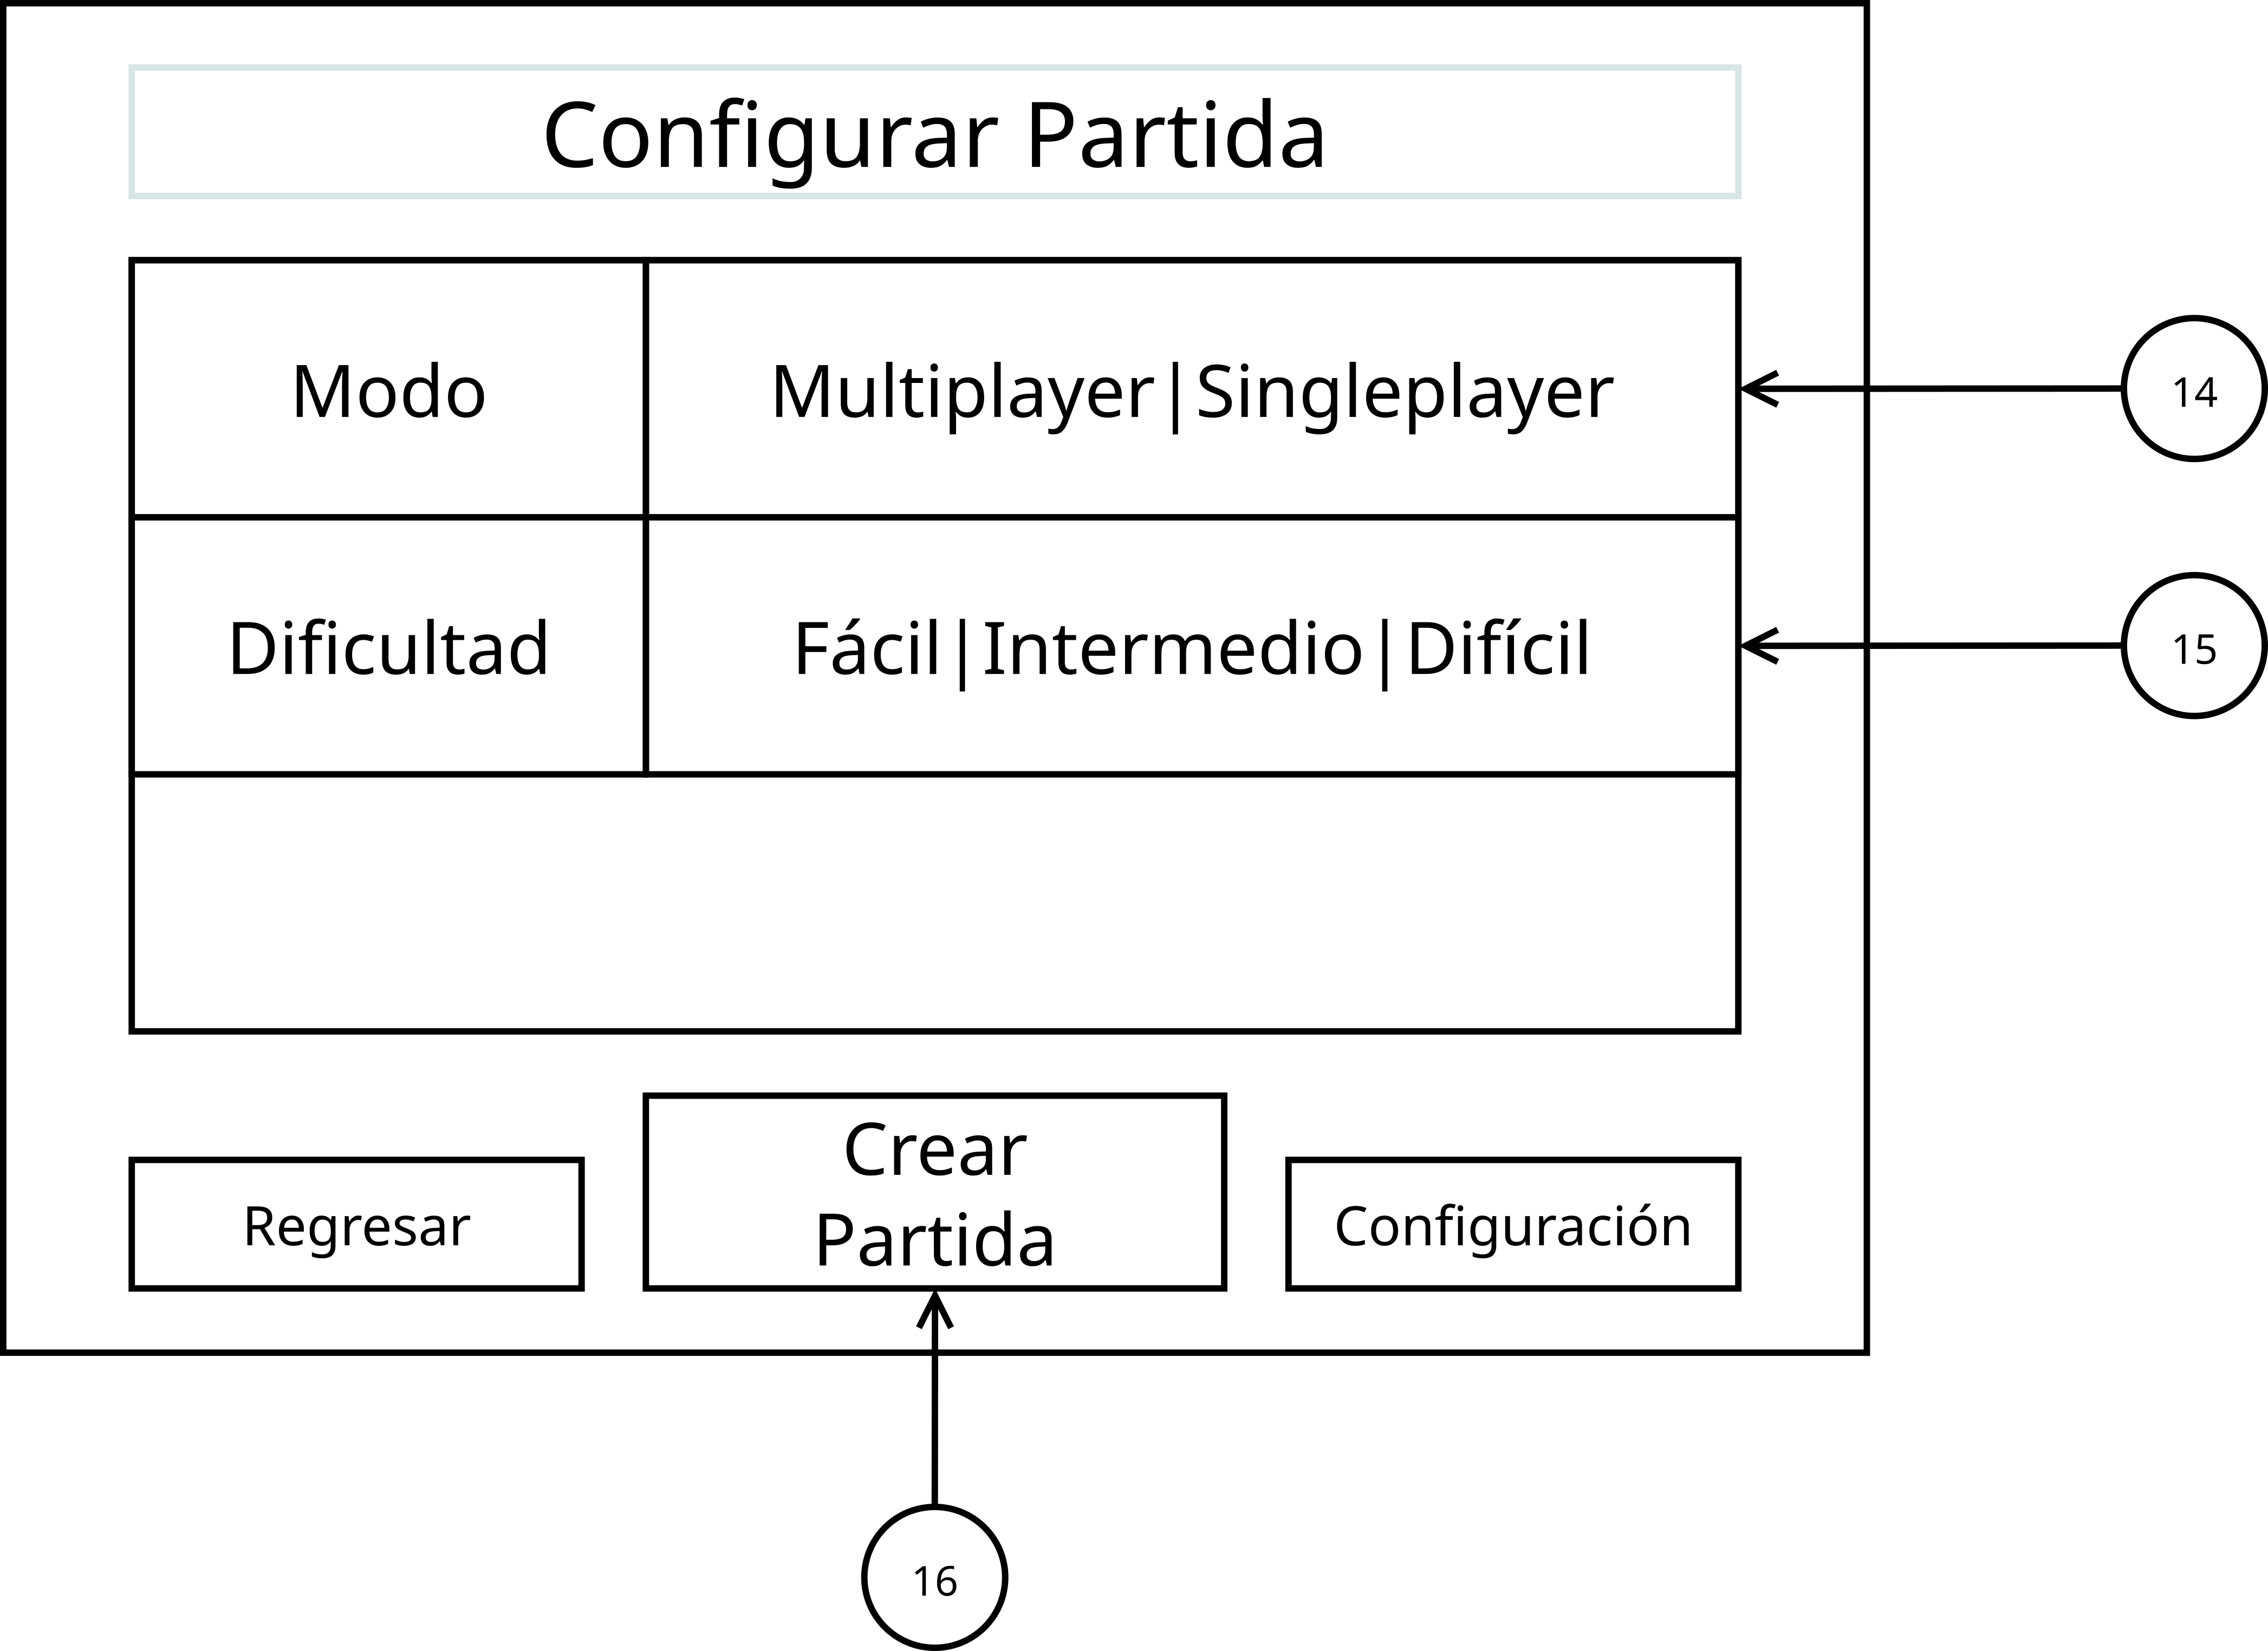
\includegraphics[width=0.5\textwidth]{5-Cuerpo/Chapter5/I4.png} %
    \caption{}
    \label{fig:I4}
\end{figure}

\subsubsection{Modo configuración de partida}
\begin{figure}[H]
    \centering
    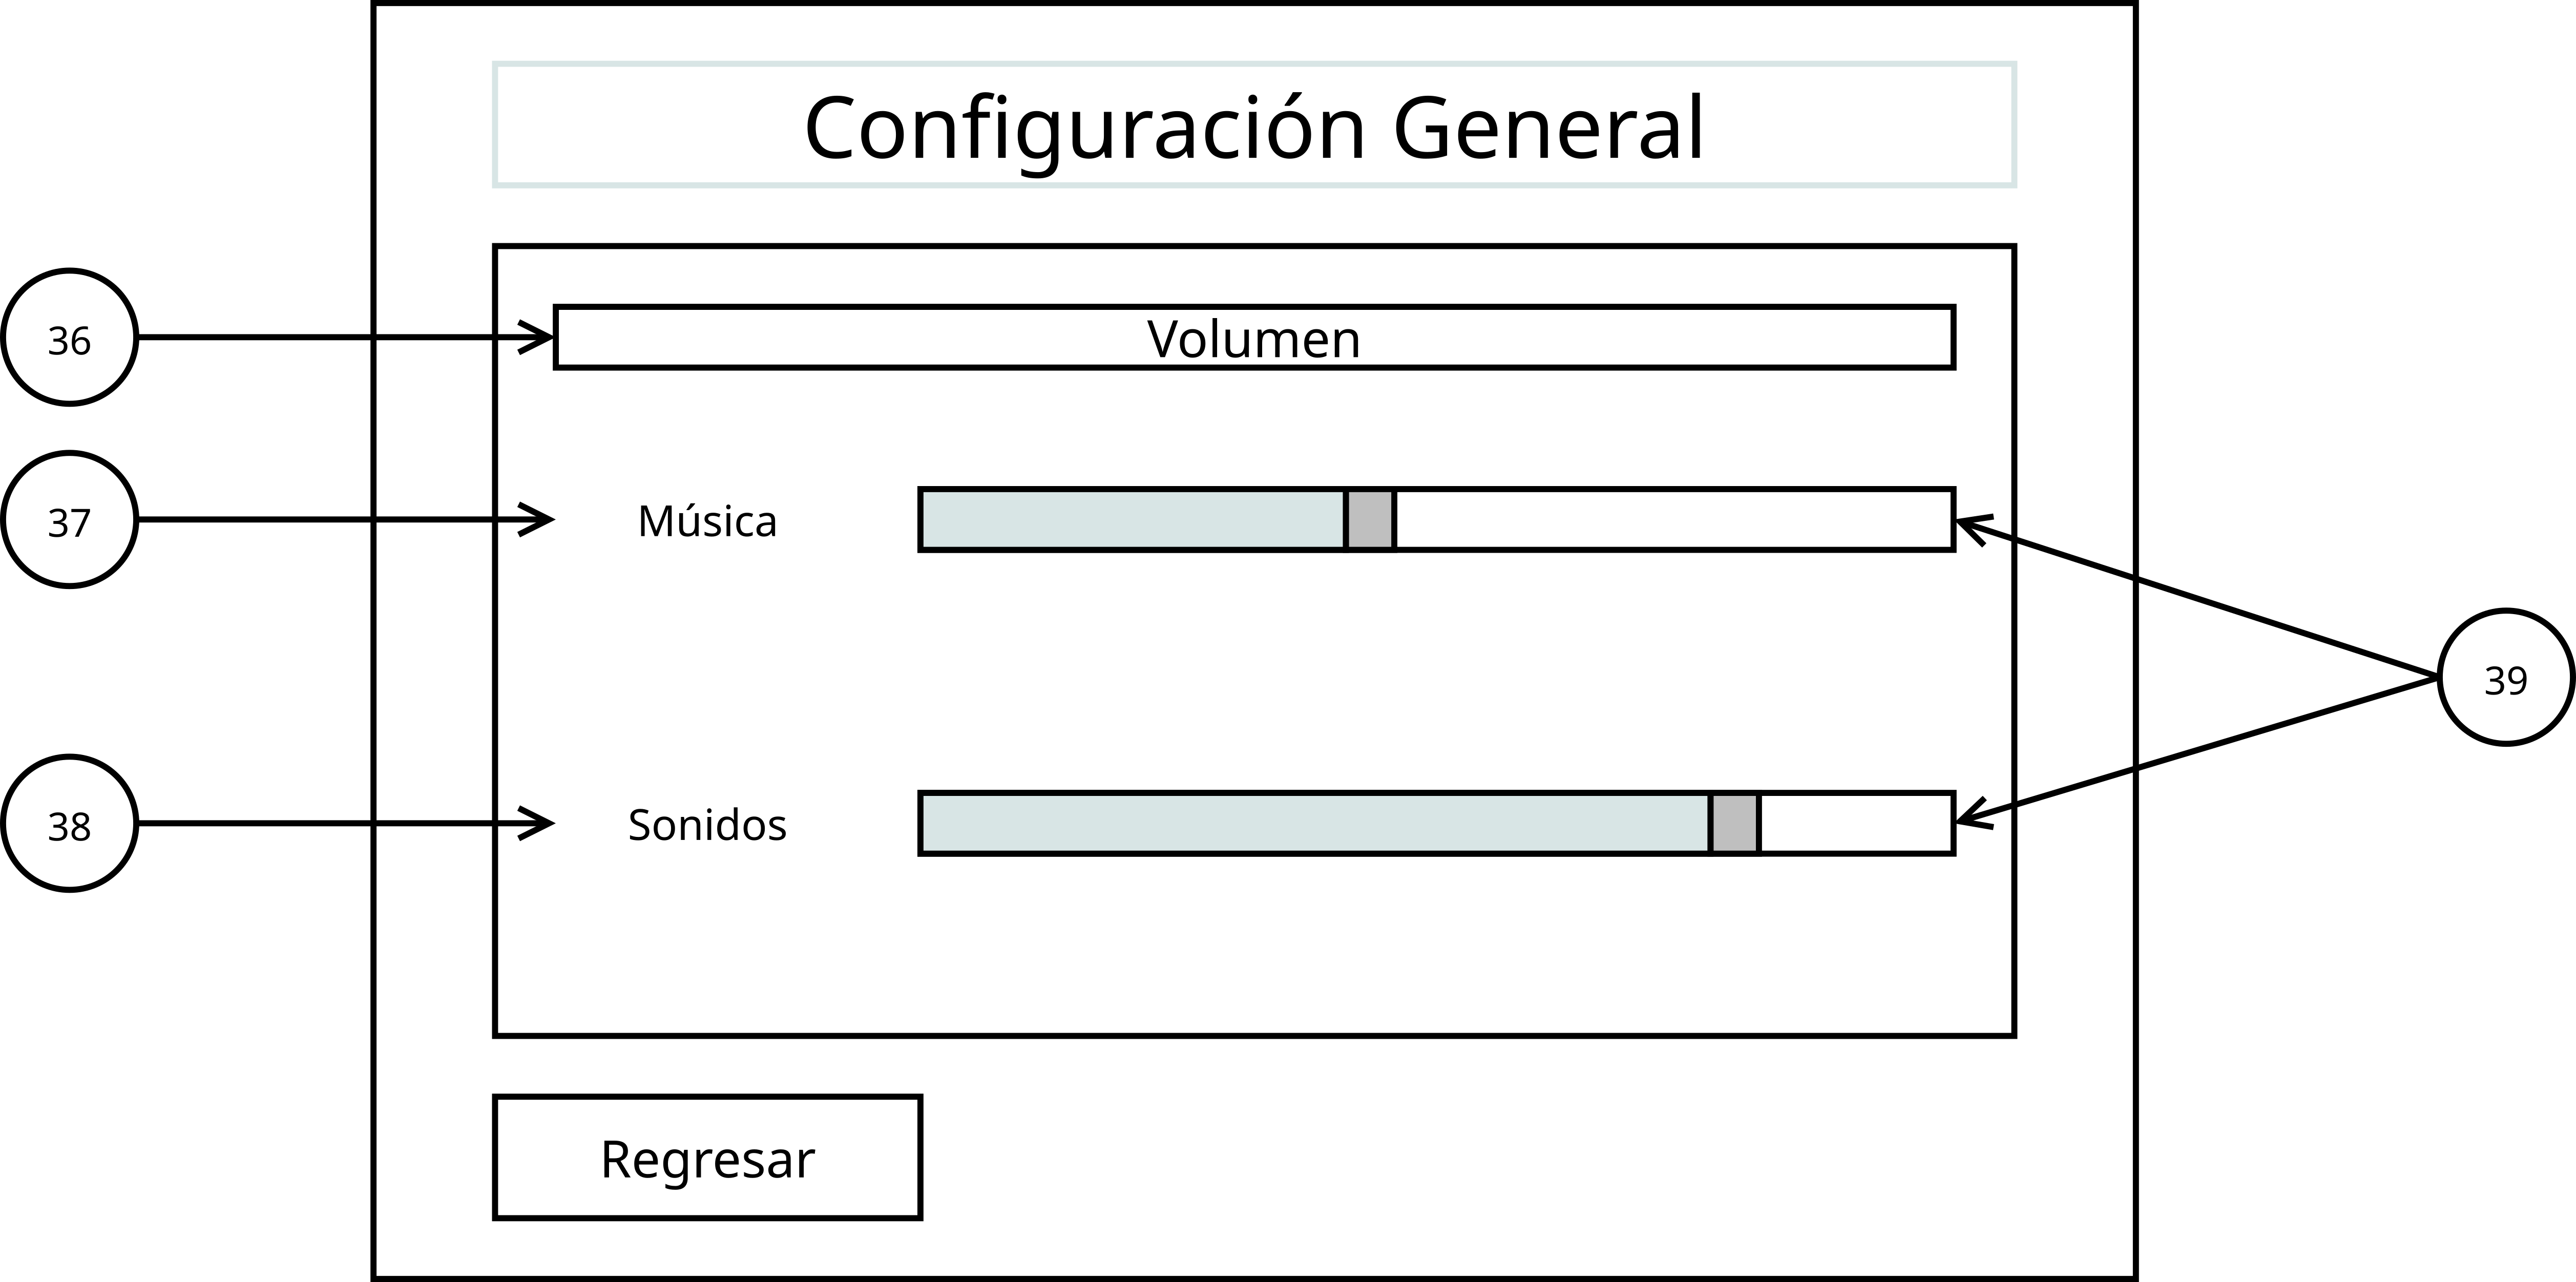
\includegraphics[width=0.5\textwidth]{5-Cuerpo/Chapter5/I10.png} %
    \caption{}
    \label{fig:I10}
\end{figure}

\subsubsection{Modo selección de personaje}
\begin{figure}[H]
    \centering
    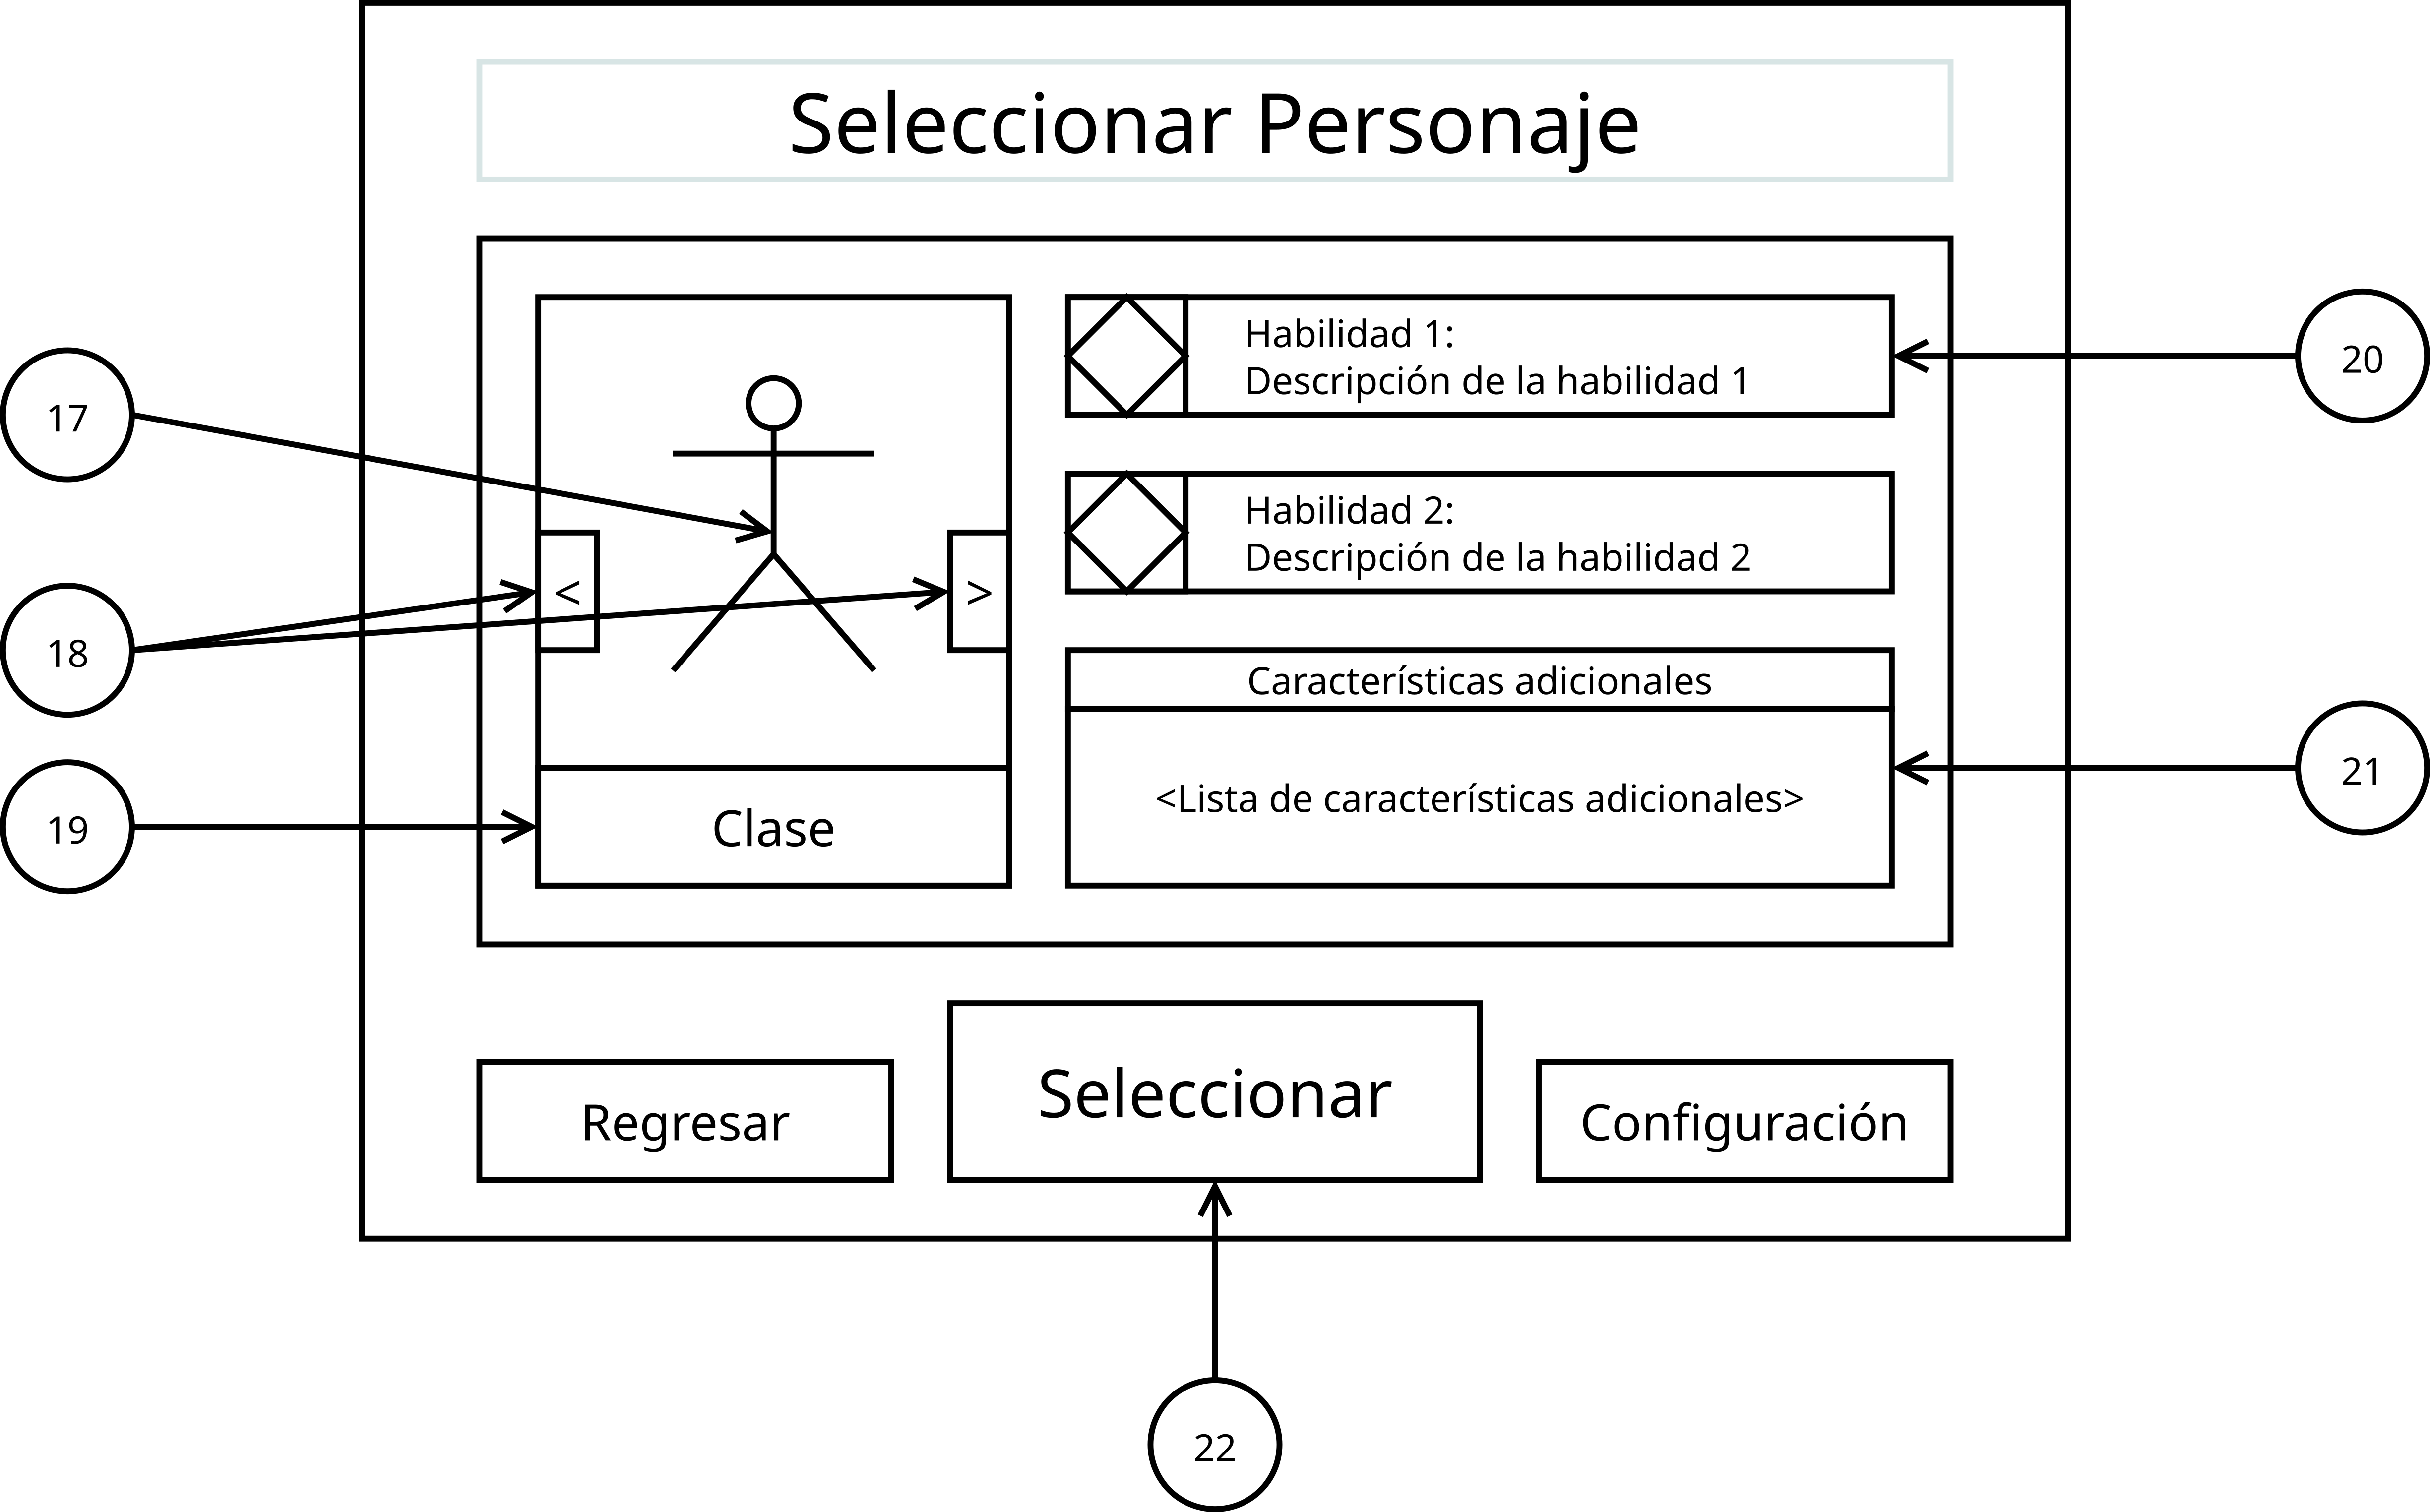
\includegraphics[width=0.5\textwidth]{5-Cuerpo/Chapter5/I5.png} %
    \caption{}
    \label{fig:I5}
\end{figure}

\subsubsection{Modo partida}
\begin{figure}[H]
    \centering
    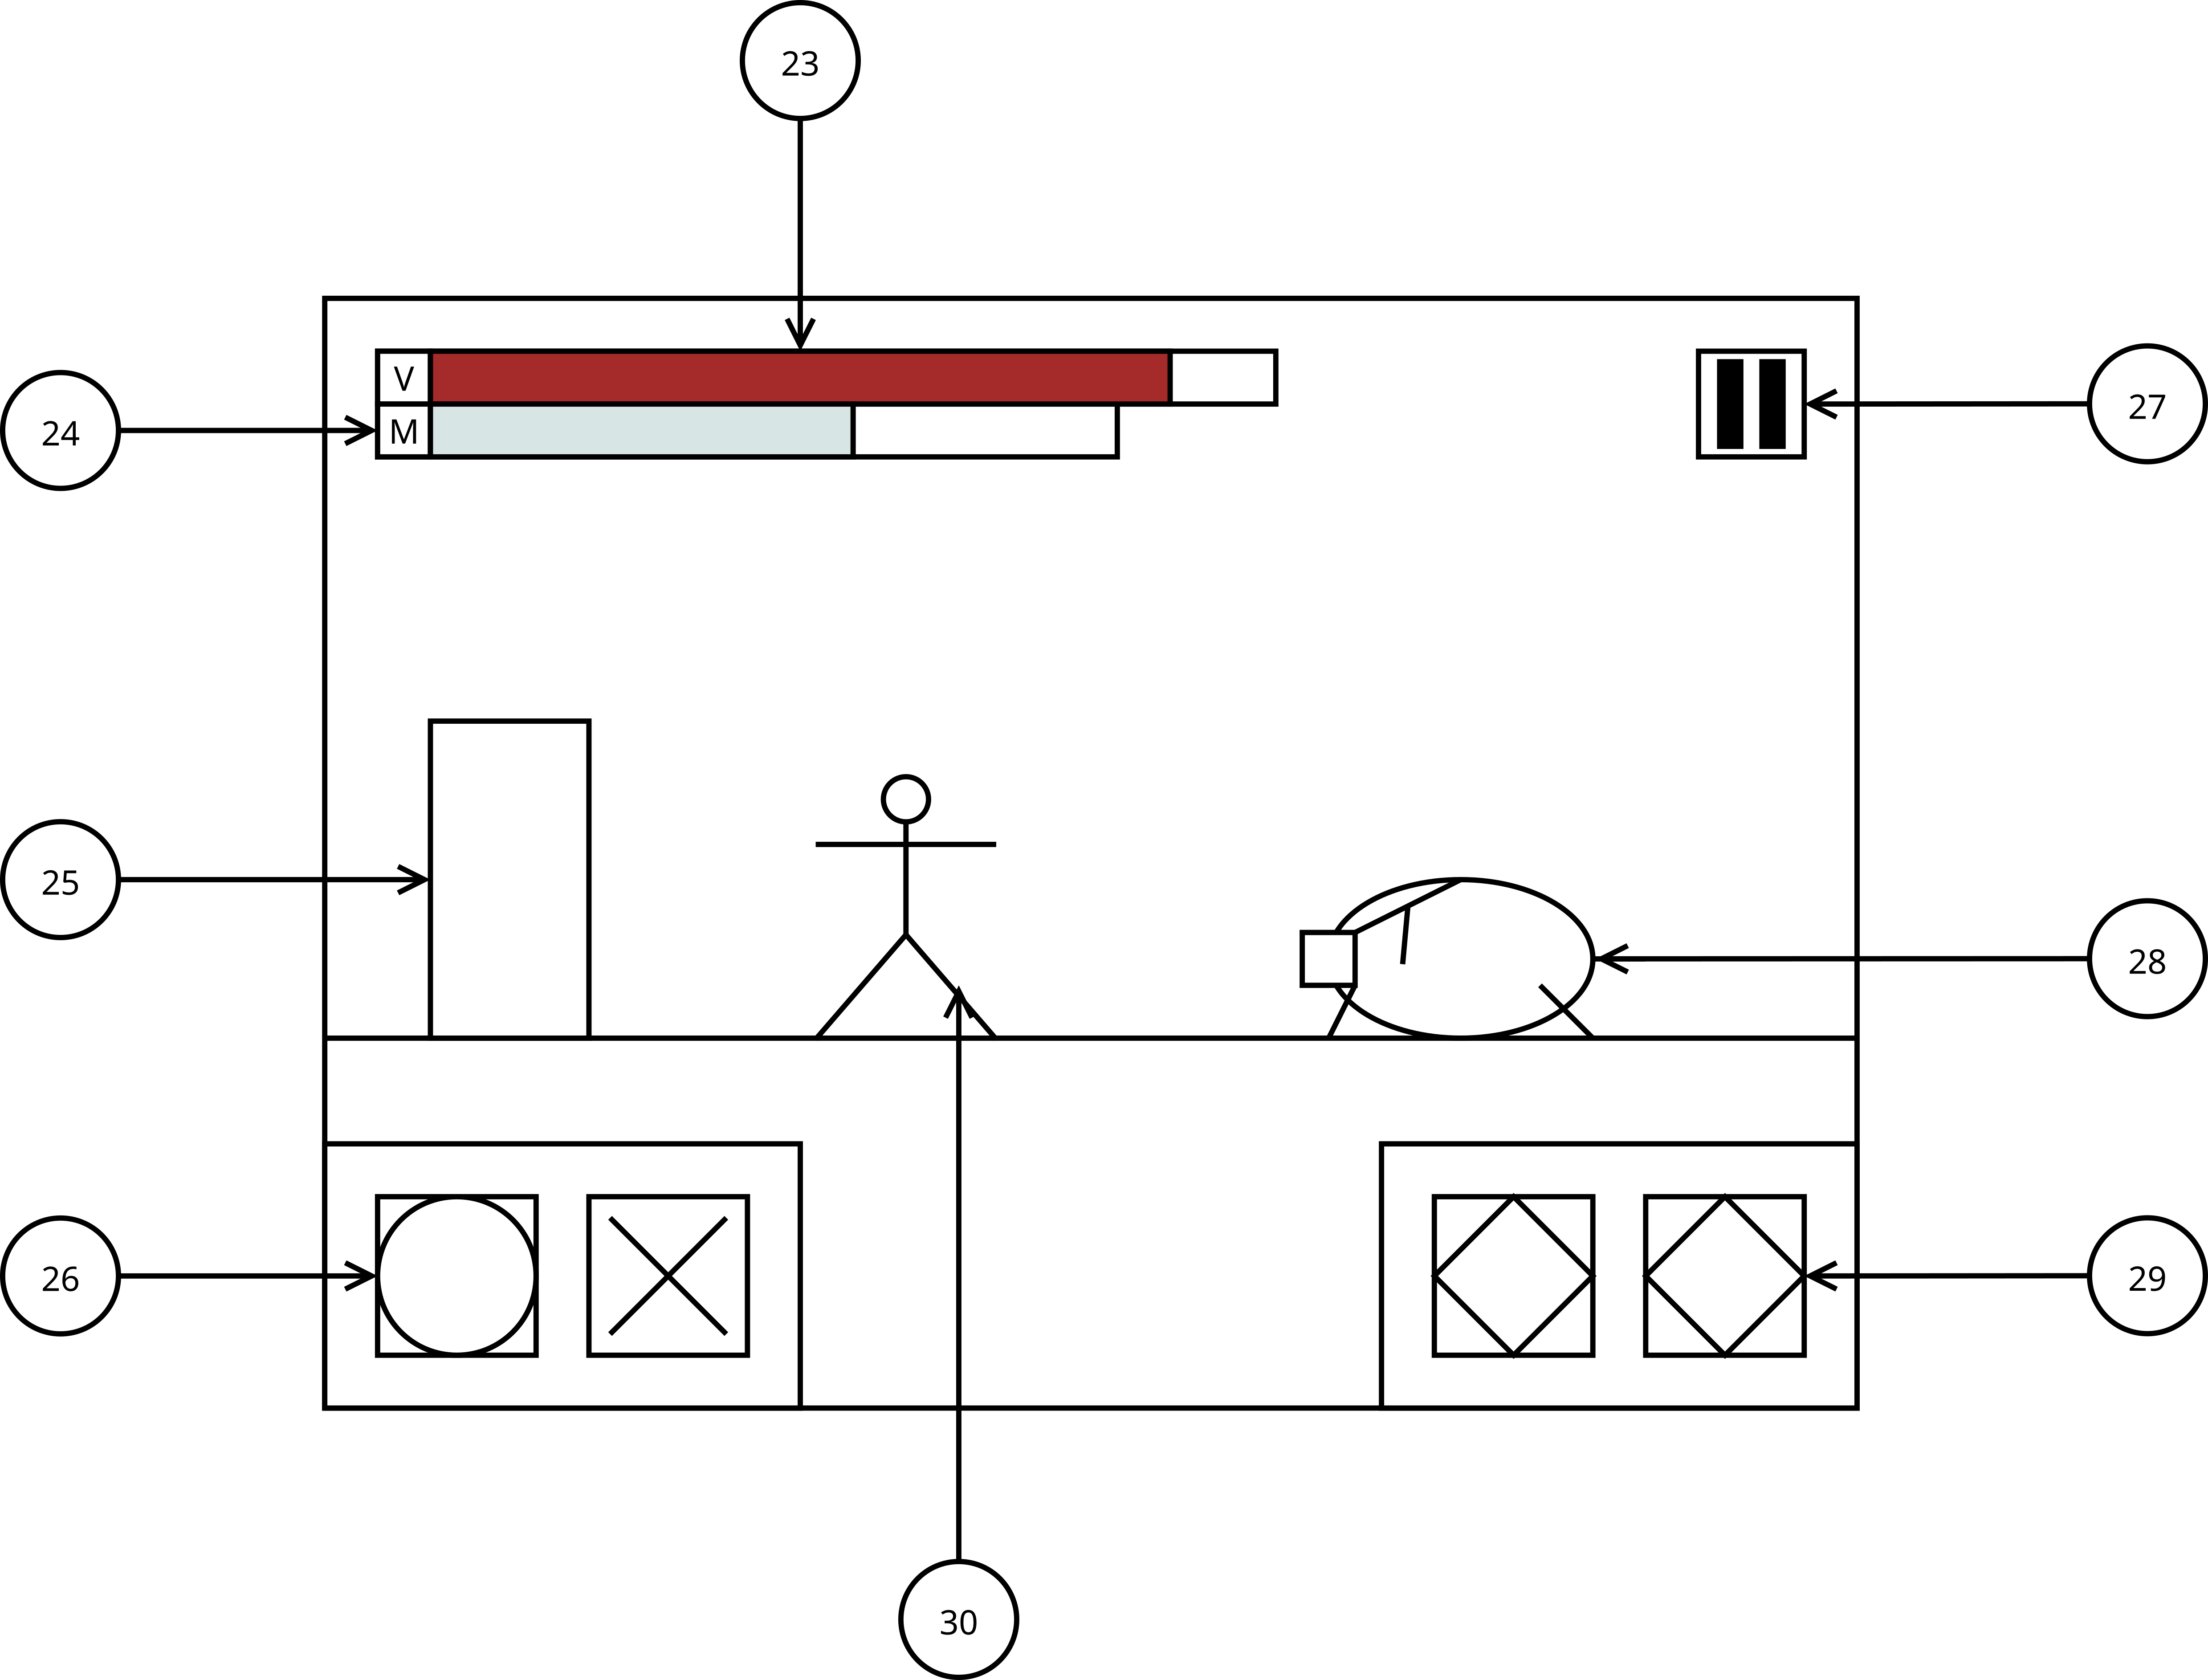
\includegraphics[width=0.5\textwidth]{5-Cuerpo/Chapter5/I6.png} %
    \caption{}
    \label{fig:I6}
\end{figure}

\subsubsection{Modo pausa}
\begin{figure}[H]
    \centering
    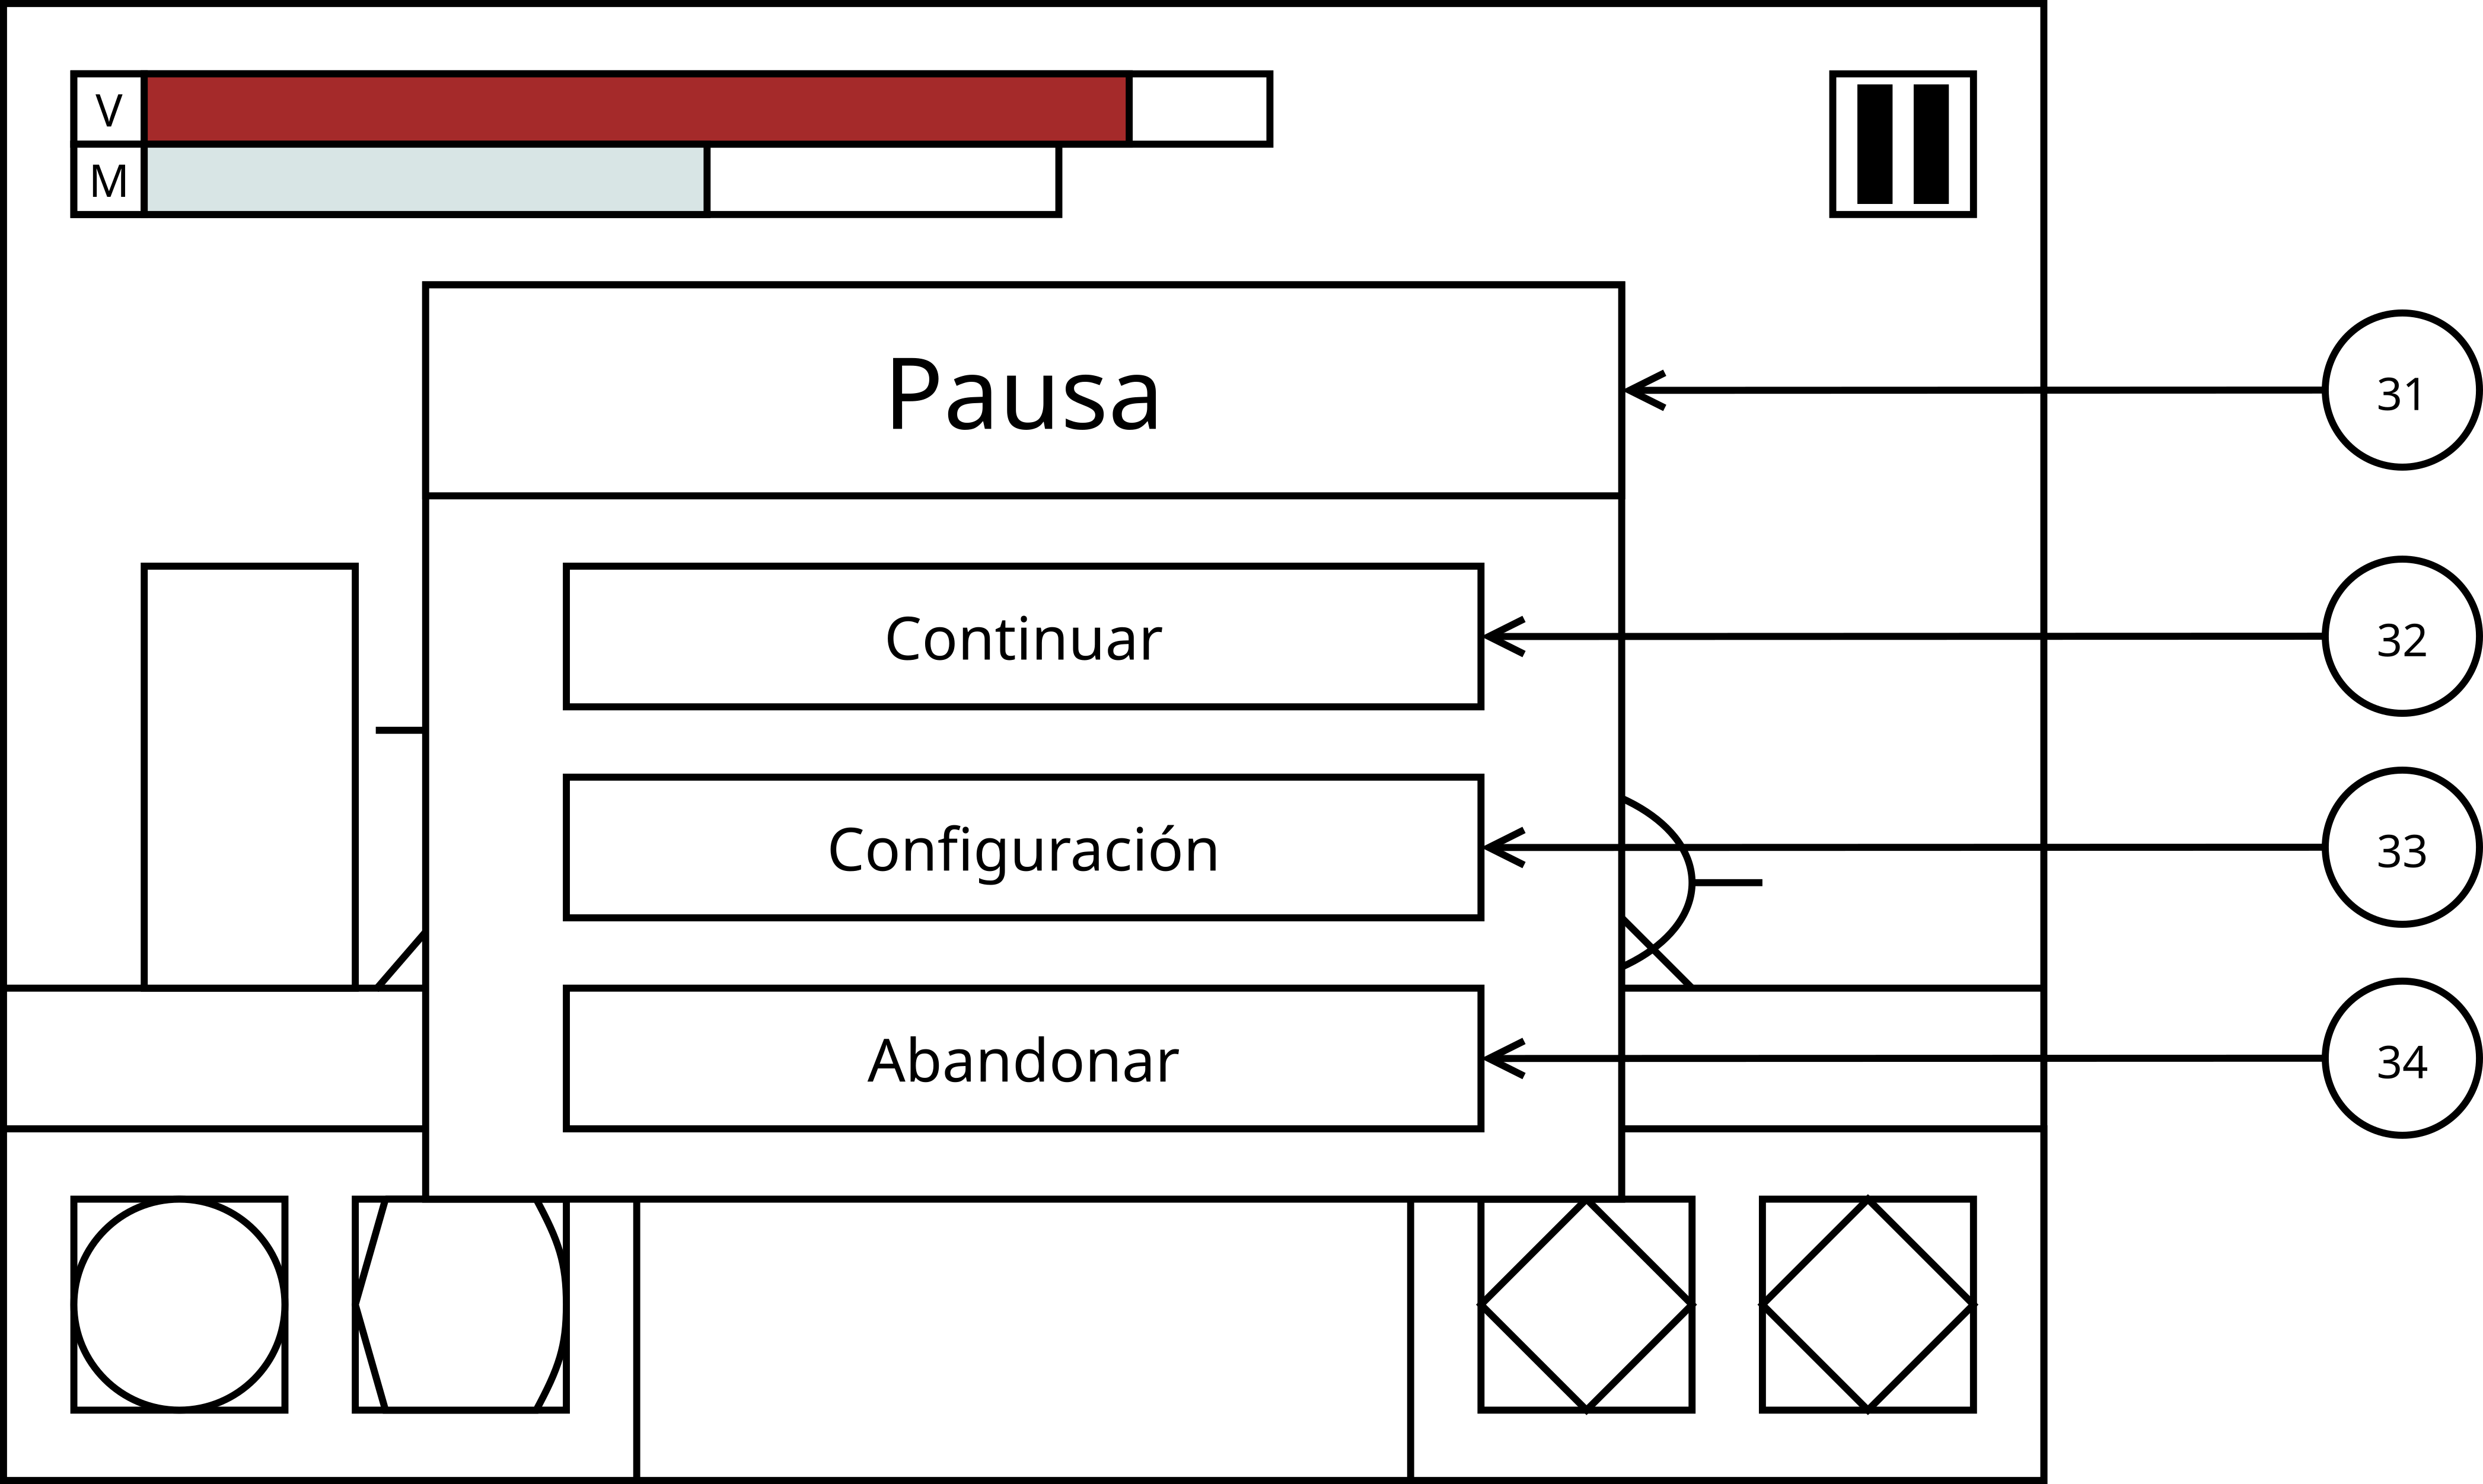
\includegraphics[width=0.5\textwidth]{5-Cuerpo/Chapter5/I7.png} %
    \caption{}
    \label{fig:I7}
\end{figure}

\subsubsection{Modo victoria}
\begin{figure}[H]
    \centering
    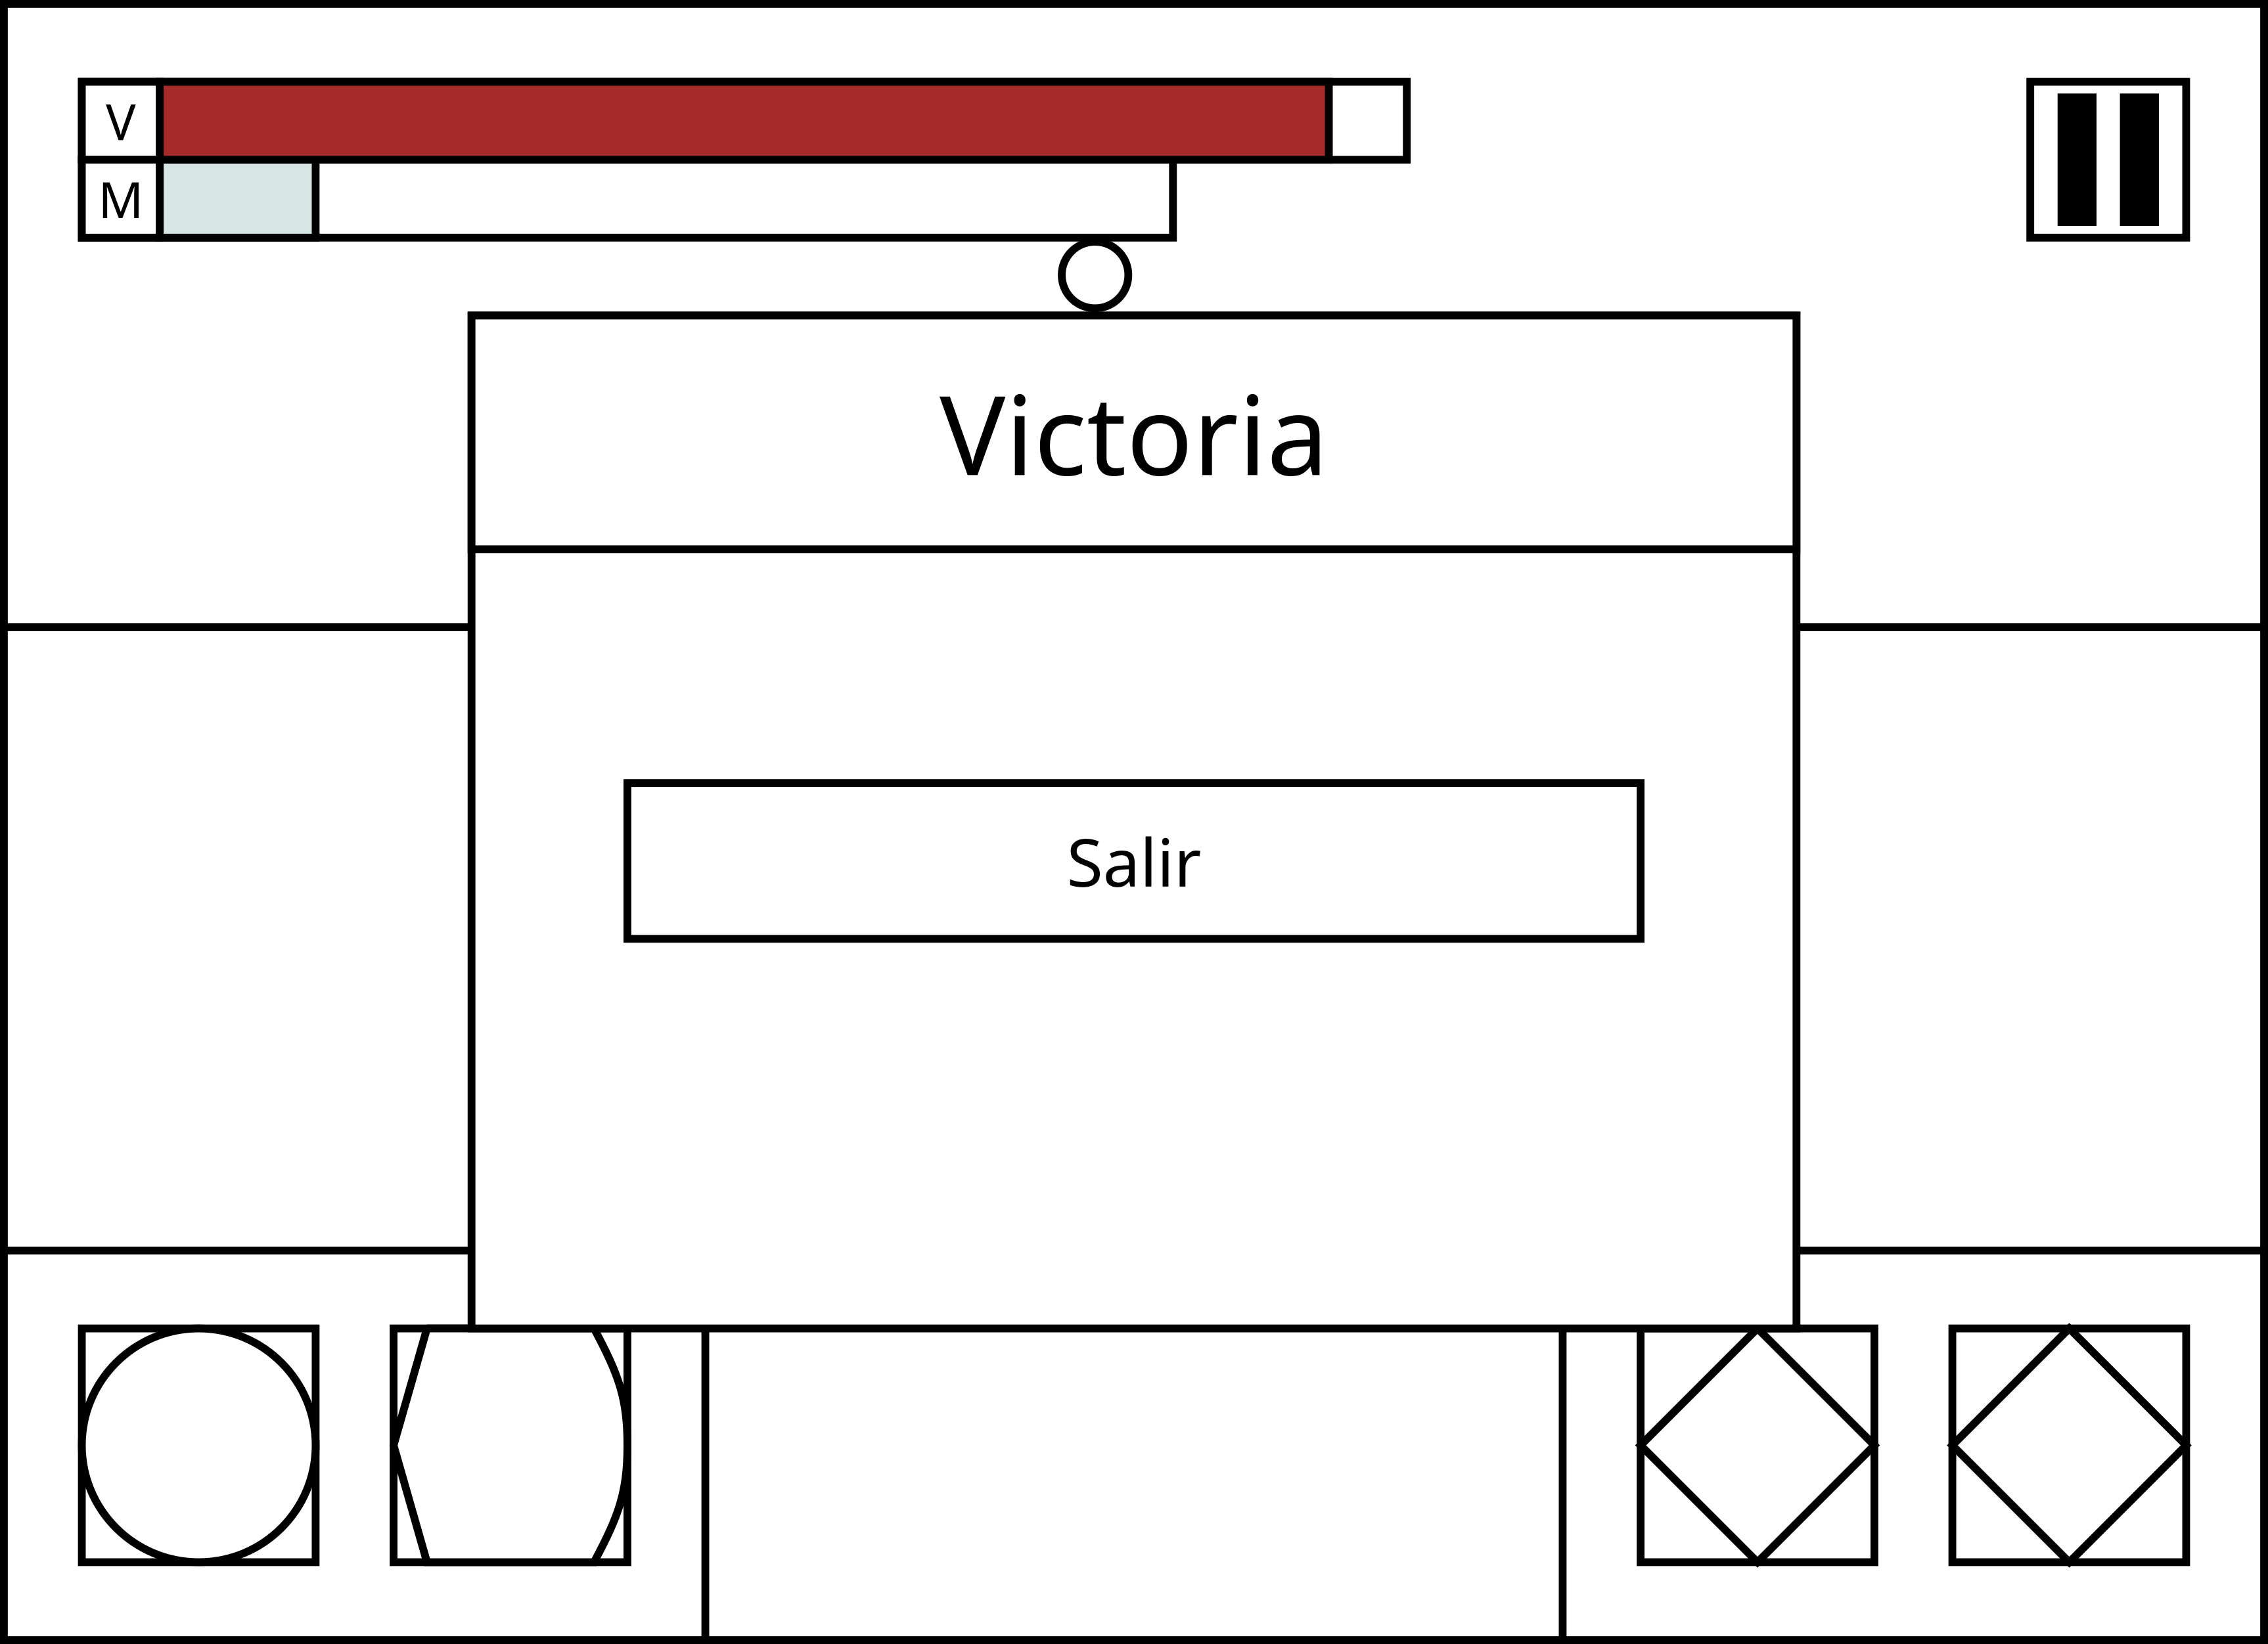
\includegraphics[width=0.5\textwidth]{5-Cuerpo/Chapter5/I9.png} %
    \caption{}
    \label{fig:I9}
\end{figure}

\subsubsection{Modo derrota}
\begin{figure}[H]
    \centering
    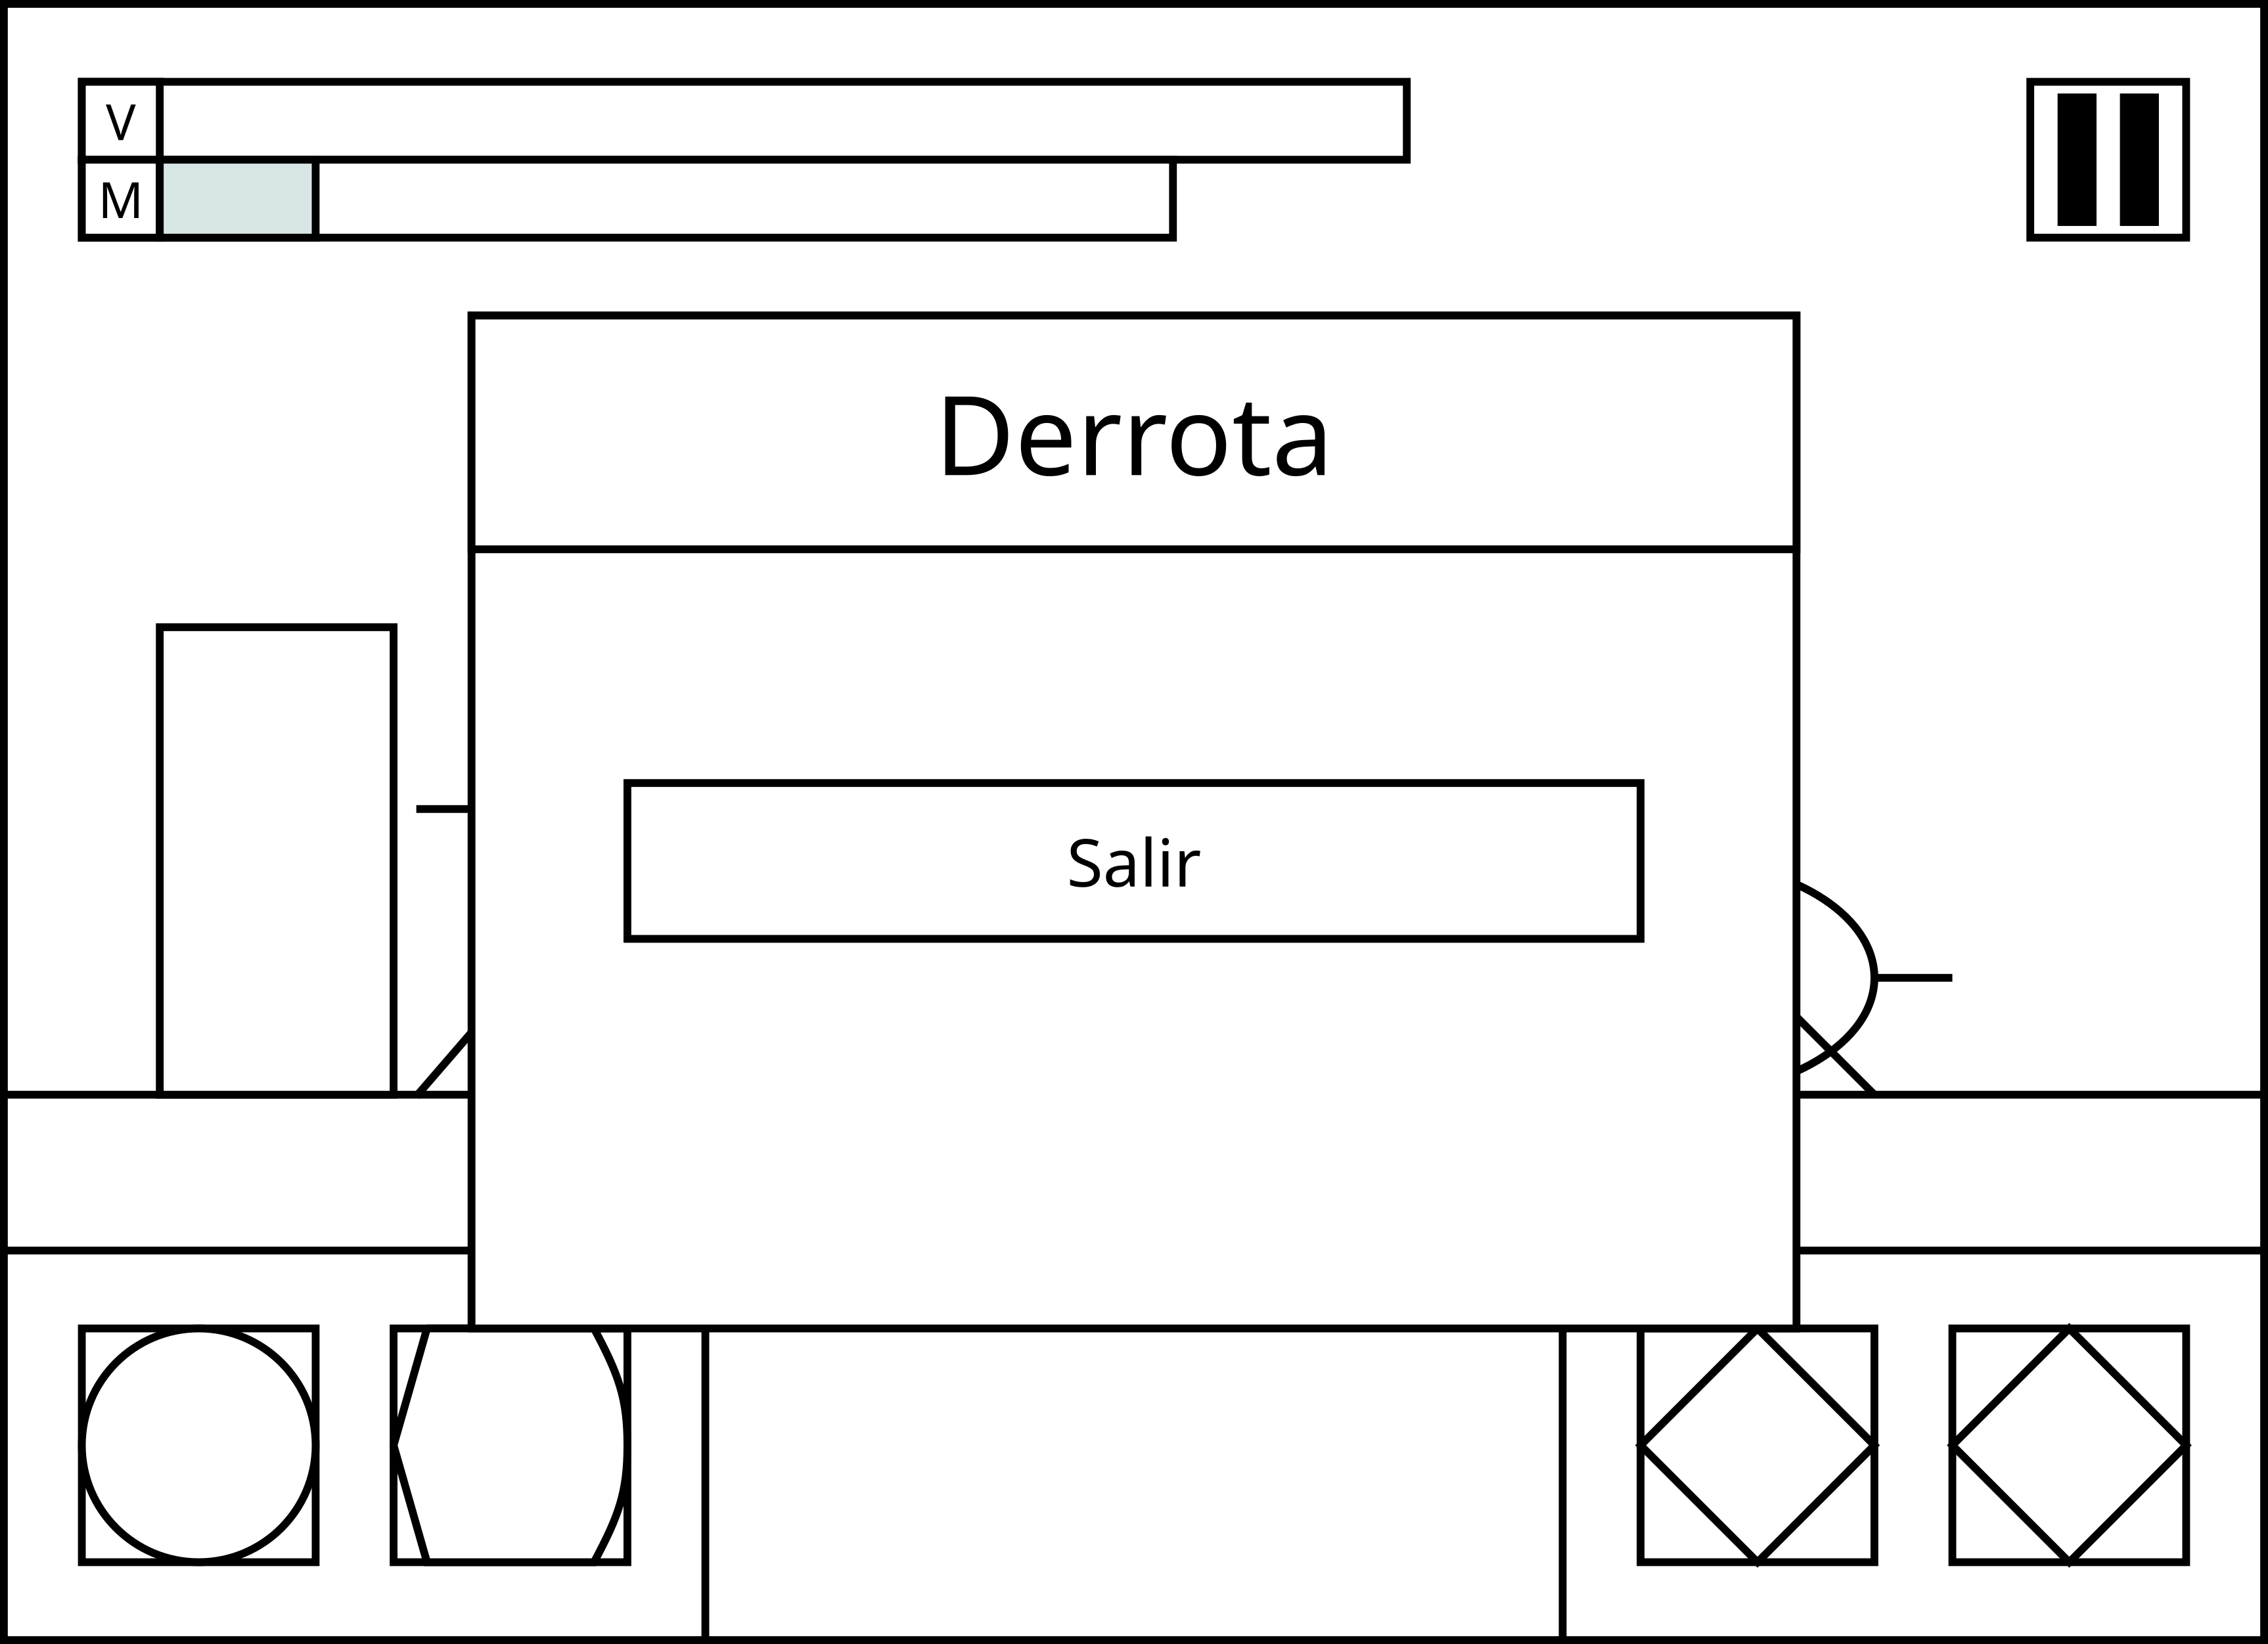
\includegraphics[width=0.5\textwidth]{5-Cuerpo/Chapter5/I8.png} %
    \caption{}
    \label{fig:I8}
\end{figure}

\subsubsection{Modo configuración}
\begin{figure}[H]
    \centering
    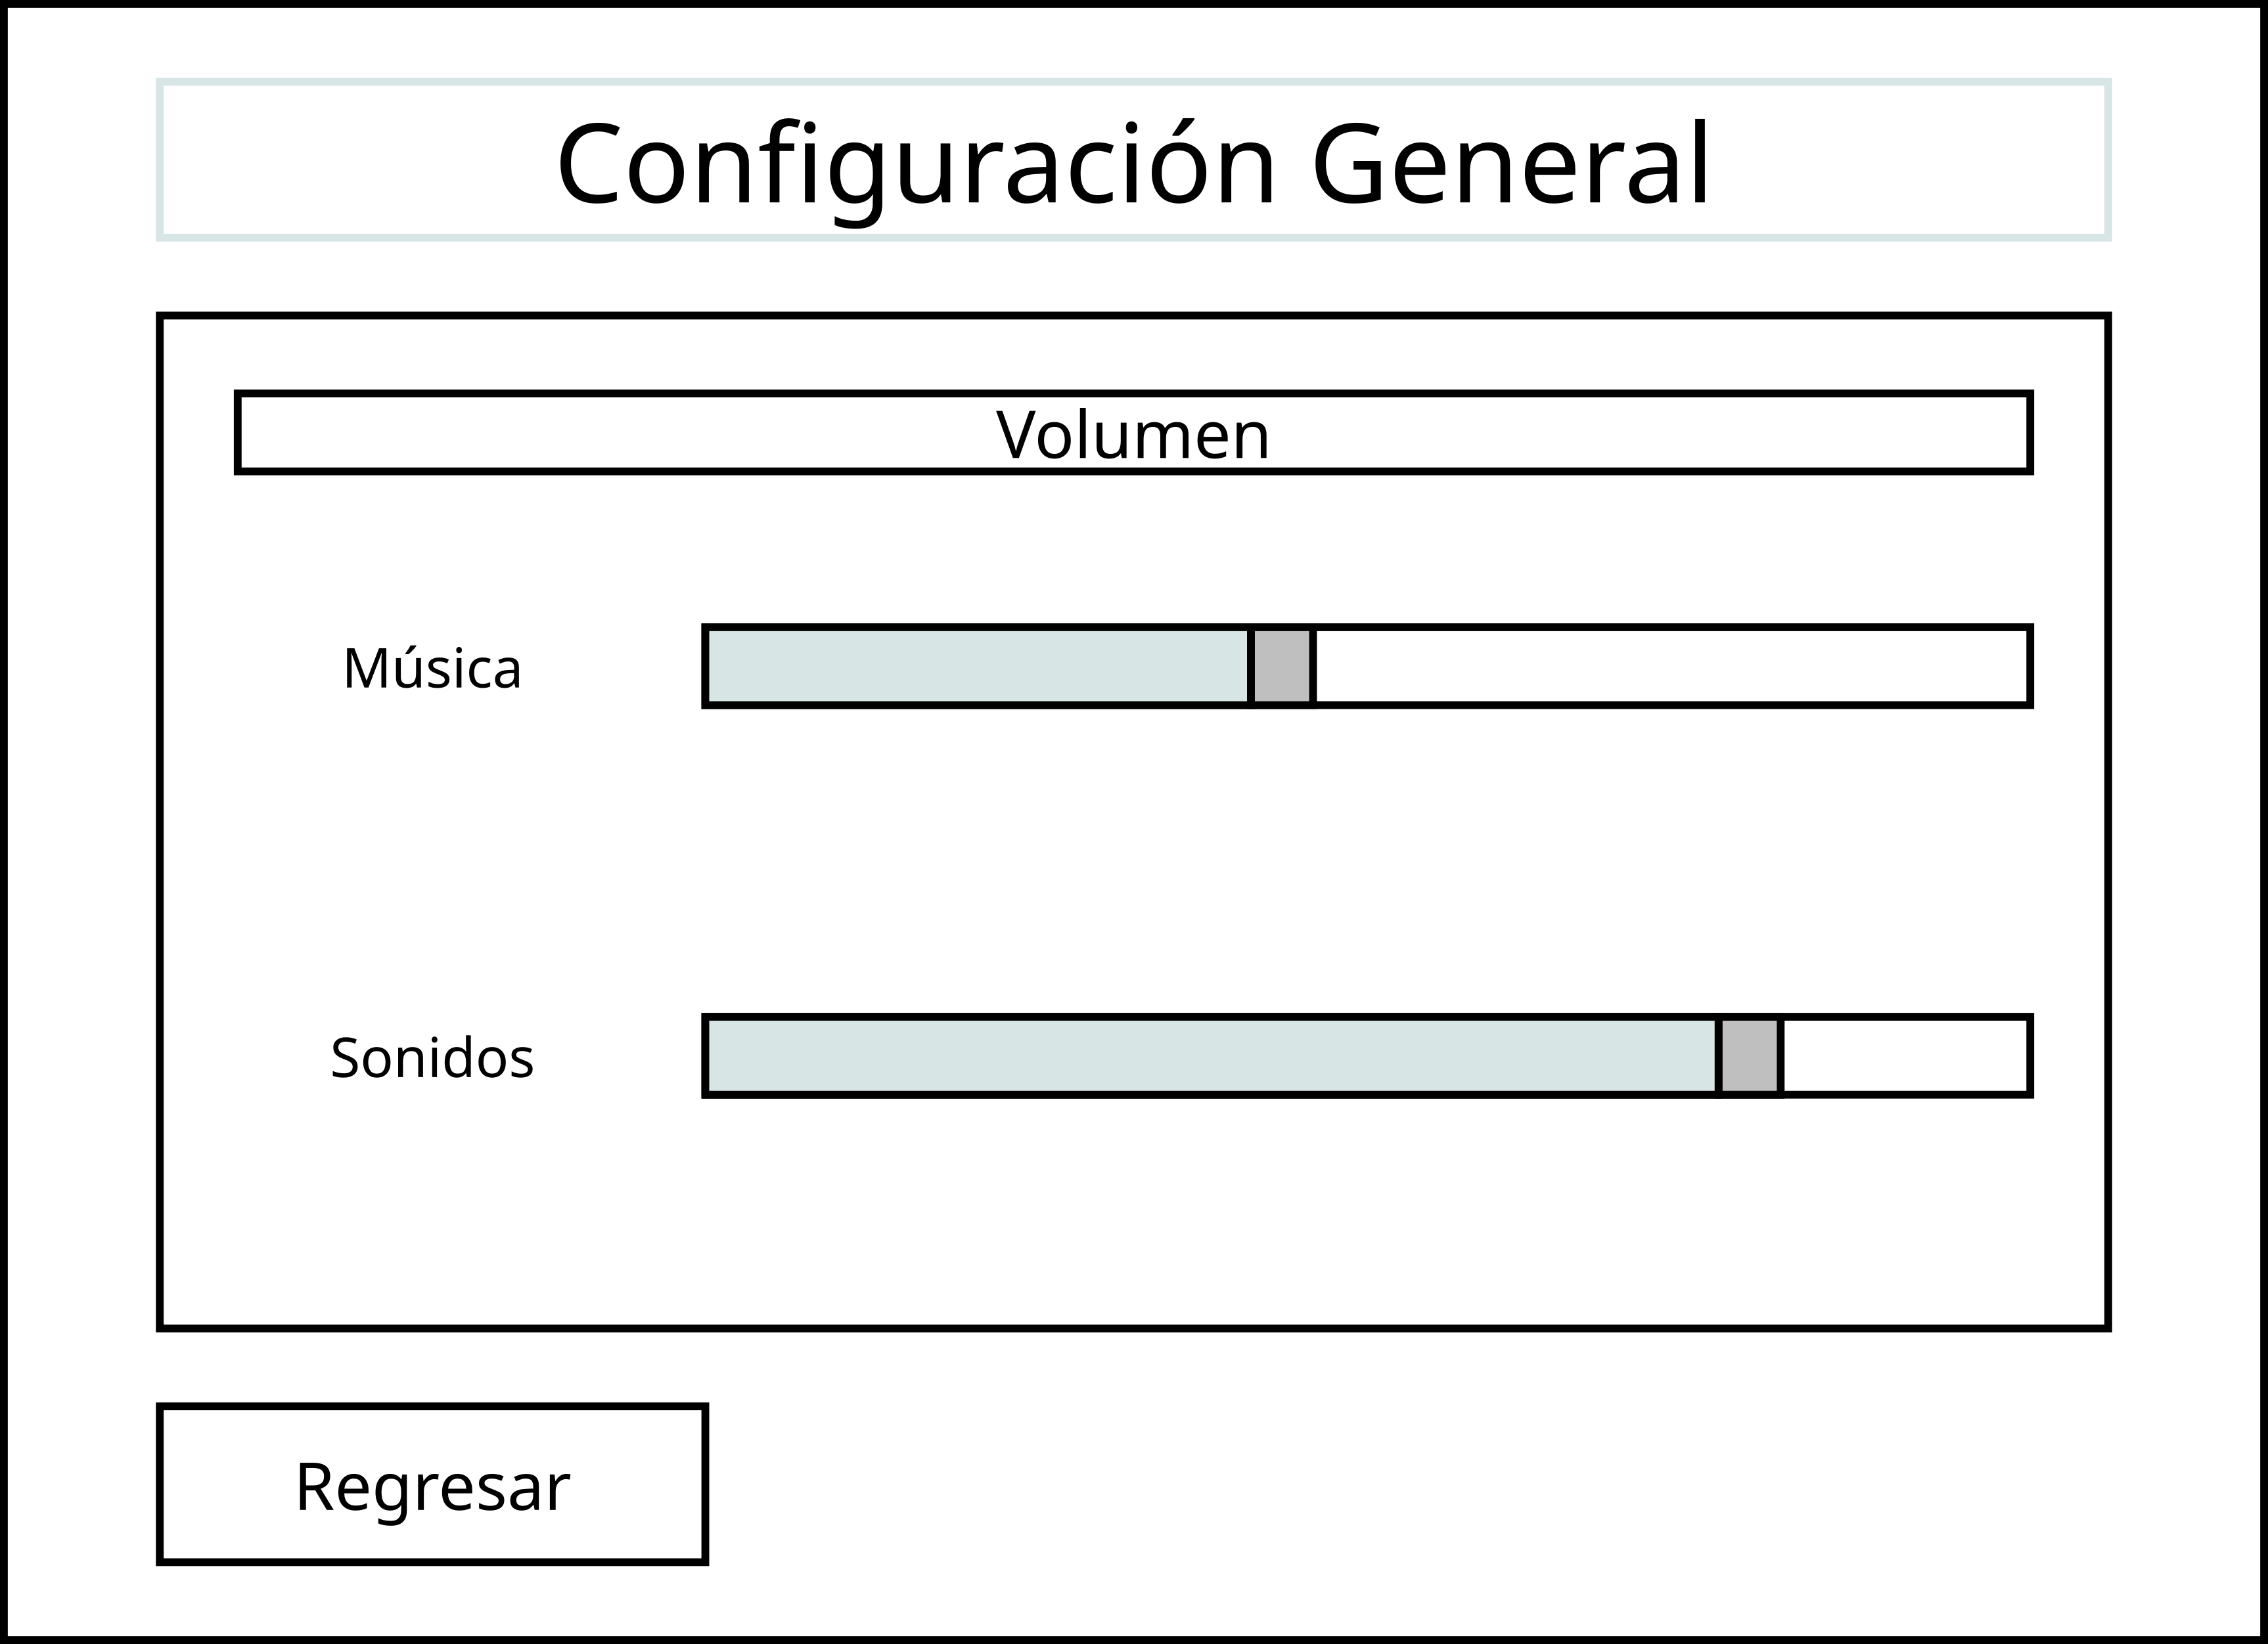
\includegraphics[width=0.5\textwidth]{5-Cuerpo/Chapter5/I2.png} %
    \caption{}
    \label{fig:I2}
\end{figure}